\documentclass[11pt,a4paper]{article}
\usepackage[utf8]{inputenc}
\usepackage[T1]{fontenc}
\usepackage{lmodern}
\usepackage[margin=2cm]{geometry}
\usepackage{amsmath,amssymb}
\usepackage{booktabs}
\usepackage{graphicx}
\usepackage{xcolor}
\usepackage{titlesec}
\usepackage{tabularx}
\usepackage{float}
\usepackage{hyperref}
\usepackage{microtype}

\hypersetup{
    colorlinks=true,
    linkcolor=blue!70!black,
    citecolor=blue!70!black,
    urlcolor=blue!70!black
}

\titleformat{\section}{\large\bfseries}{\thesection.}{0.5em}{}
\titleformat{\subsection}{\normalsize\bfseries}{\thesubsection.}{0.5em}{}
\titlespacing*{\section}{0pt}{1.2ex plus 0.5ex minus .2ex}{0.6ex}
\titlespacing*{\subsection}{0pt}{1.0ex plus 0.4ex minus .2ex}{0.4ex}

\setlength{\parskip}{0.45em}
\setlength{\parindent}{0pt}

\begin{document}

\begin{center}
    {\LARGE \textbf{Projeto 2: Quantização de Cores com Redes SOM e GNG}} \\[0.35em]
    {\large Disciplina: Introdução às Redes Neurais Artificiais} \\[0.3em]
    \textbf{Autor:} Gabriel Bonavina (RA: 168.858)\\[0.2em]
    \textbf{Repositório:} \url{https://github.com/gbonavina/projeto-2-rna}
\end{center}
\vspace{-0.5em}
\hrule
\vspace{0.8em}

\section*{Configuração Experimental}

Este trabalho analisa a compressão e redução do espaço de cores de cinco imagens digitais por meio de dois paradigmas clássicos de aprendizado competitivo não supervisionado: os Mapas Auto-Organizáveis de Kohonen (\textit{Self-Organizing Maps} -- SOM) e o \textit{Growing Neural Gas} (GNG). Em ambos os modelos, o problema é formulado de maneira equivalente: cada pixel no espaço de cores RGB é tratado como um vetor de entrada $\mathbf{x} \in [0, 1]^3$. Ao término do treinamento, o conjunto de protótipos (pesos sinápticos) converge para o \textit{codebook} da paleta quantizada, e a imagem reconstruída é obtida associando-se cada pixel ao protótipo de menor distância euclidiana:
\begin{equation}
    c(\mathbf{x}) = \arg\min_{i} \|\mathbf{x} - \mathbf{w}_i\|_2
\end{equation}

O conjunto de dados, disponível no diretório \texttt{data/}, é composto por fotografias de alta resolução: quatro com dimensões originais de $4032 \times 3024$ pixels (\texttt{image1}, \texttt{image2}, \texttt{image4} e \texttt{image5}) e uma de $4032 \times 2268$ pixels (\texttt{image3}). Visando a padronização experimental e viabilidade computacional, todas as imagens foram convertidas para RGB e redimensionadas para $450 \times 450$ pixels através de reamostragem com filtro Lanczos, gerando $N = 202\,500$ amostras por imagem. A complexidade espectral resultante varia entre $55\,122$ cores distintas em \texttt{image5} e $88\,833$ em \texttt{image4}.

A reprodutibilidade foi garantida fixando a semente pseudoaleatória em $42$. Foram avaliados codebooks de cardinalidade $K \in \{16, 64, 256\}$, que no caso da SOM correspondem a topologias bidimensionais de $4 \times 4$, $8 \times 8$ e $16 \times 16$ neurônios. O desempenho foi quantificado por meio de três métricas analíticas:
\begin{enumerate}
    \item \textbf{Erro Médio de Quantização (QE):} distância euclidiana média entre os pixels originais e os respectivos protótipos mais próximos no espaço normalizado $[0, 1]^3$;
    \item \textbf{Erro Quadrático Médio (MSE):} média das distâncias euclidianas quadradas nos três canais normalizados;
    \item \textbf{Pico da Relação Sinal-Ruído (PSNR):} expresso em decibéis (dB) por $\mathrm{PSNR} = 10 \log_{10}(1/\mathrm{MSE})$.
\end{enumerate}

Adicionalmente, contabilizou-se a eficiência do uso do codebook mensurando o número de protótipos efetivamente distintos após quantização e arredondamento para a faixa clássica de $8$ bits por canal ($[0, 255]$), o que expõe eventuais colapsos de neurônios para tons redundantes.
\section{Mapas Auto-Organizáveis (SOM)}

O treinamento da SOM baseou-se na biblioteca de aceleração matricial \textit{XPySom}, operando em espaço tridimensional ao longo de $100$ épocas completas. A cada época, todos os $202\,500$ pixels foram apresentados, totalizando $20{,}25 \times 10^6$ passos de atualização por grade. A taxa de aprendizado inicial $\eta_0 = 0{,}5$ decaiu exponencialmente até $\eta_N = 0{,}01$. A dinâmica de vizinhança gaussiana adotou como raio inicial metade da extensão lateral da grade ($\sigma_0 = 2$, $4$ e $8$ para $4 \times 4$, $8 \times 8$ e $16 \times 16$, respectivamente), decaindo monotonicamente até $\sigma_N = 1{,}0$. A topologia retangular e a largura intrínseca $\mathrm{std} = 0{,}5$ seguiram as diretrizes padrão da biblioteca.

A escolha de $\sigma_0$ assegura uma cobertura ampla no início do processo, forçando unidades adjacentes na grade a convergirem para regiões conexas do espaço de cores e preservando as relações topológicas. Conforme $\sigma \to 1{,}0$, o acoplamento lateral enfraquece, permitindo o refinamento individual de cada protótipo.

\begin{table}[H]
\centering
\caption{Métricas obtidas com o modelo SOM após quantização para $8$ bits.}
\label{tab:som}
\small
\begin{tabular}{llrrrr}
\toprule
Imagem & Grade & Erro de Quant. & MSE & PSNR (dB) & Cores Efetivas \\
\midrule
image1 & $4 \times 4$   & 0,0691 & $2{,}45 \times 10^{-3}$ & 26,10 & 16 \\
image1 & $8 \times 8$   & 0,0348 & $6{,}87 \times 10^{-4}$ & 31,63 & 64 \\
image1 & $16 \times 16$ & 0,0194 & $2{,}19 \times 10^{-4}$ & 36,59 & 256 \\
\midrule
image2 & $4 \times 4$   & 0,0620 & $1{,}76 \times 10^{-3}$ & 27,54 & 16 \\
image2 & $8 \times 8$   & 0,0322 & $5{,}06 \times 10^{-4}$ & 32,96 & 63 \\
image2 & $16 \times 16$ & 0,0175 & $1{,}46 \times 10^{-4}$ & 38,34 & 254 \\
\midrule
image3 & $4 \times 4$   & 0,0591 & $1{,}52 \times 10^{-3}$ & 28,18 & 16 \\
image3 & $8 \times 8$   & 0,0281 & $3{,}77 \times 10^{-4}$ & 34,24 & 63 \\
image3 & $16 \times 16$ & 0,0152 & $1{,}19 \times 10^{-4}$ & 39,26 & 250 \\
\midrule
image4 & $4 \times 4$   & 0,0666 & $2{,}05 \times 10^{-3}$ & 26,88 & 16 \\
image4 & $8 \times 8$   & 0,0317 & $5{,}52 \times 10^{-4}$ & 32,58 & 63 \\
image4 & $16 \times 16$ & 0,0169 & $1{,}62 \times 10^{-4}$ & 37,90 & 254 \\
\midrule
image5 & $4 \times 4$   & 0,0444 & $1{,}07 \times 10^{-3}$ & 29,72 & 16 \\
image5 & $8 \times 8$   & 0,0238 & $3{,}52 \times 10^{-4}$ & 34,53 & 64 \\
image5 & $16 \times 16$ & 0,0132 & $1{,}22 \times 10^{-4}$ & 39,12 & 256 \\
\midrule
Média  & $4 \times 4$   & 0,0602 & $1{,}77 \times 10^{-3}$ & 27,68 & 16,0 \\
Média  & $8 \times 8$   & 0,0301 & $4{,}95 \times 10^{-4}$ & 33,19 & 63,4 \\
Média  & $16 \times 16$ & 0,0164 & $1{,}54 \times 10^{-4}$ & 38,24 & 254,0 \\
\bottomrule
\end{tabular}
\end{table}

A expansão da malha resulta em ganhos substanciais de fidelidade: dobrar a dimensão lateral reduz o erro de quantização aproximadamente pela metade em todos os casos. O PSNR médio ascende de $27{,}68\,\mathrm{dB}$ ($16$ cores) para $33{,}19\,\mathrm{dB}$ ($64$ cores) e $38{,}24\,\mathrm{dB}$ ($256$ cores). Perceptualmente, a quantização com $16$ cores introduz artefatos severos de posterização (\textit{color banding}) em gradientes suaves como céus; a configuração com $64$ protótipos mitiga grande parte das transições bruscas; por fim, $256$ cores proporcionam reconstruções praticamente indistinguíveis do original a olho nu.

A rigidez topológica imposta pelo SOM converte a grade neural em um mapa bidimensional estruturado do espaço de cores da fotografia. Em \texttt{image1} (Figura~\ref{fig:som-1}), observa-se a transição contínua entre o amarelo solar em um vértice, os tons de azul ao longo da borda superior e sombras escuras no canto oposto. Em contrapartida, essa atração elástica lateral pode provocar o colapso de protótipos em resoluções discretizadas ($8$ bits): nas configurações $8 \times 8$ e $16 \times 16$ de \texttt{image2}, \texttt{image3} e \texttt{image4}, o número de cores distintas foi sutilmente inferior ao total de neurônios (e.g., $250$ cores para $256$ neurônios em \texttt{image3}).

\begin{figure}[H]
\centering
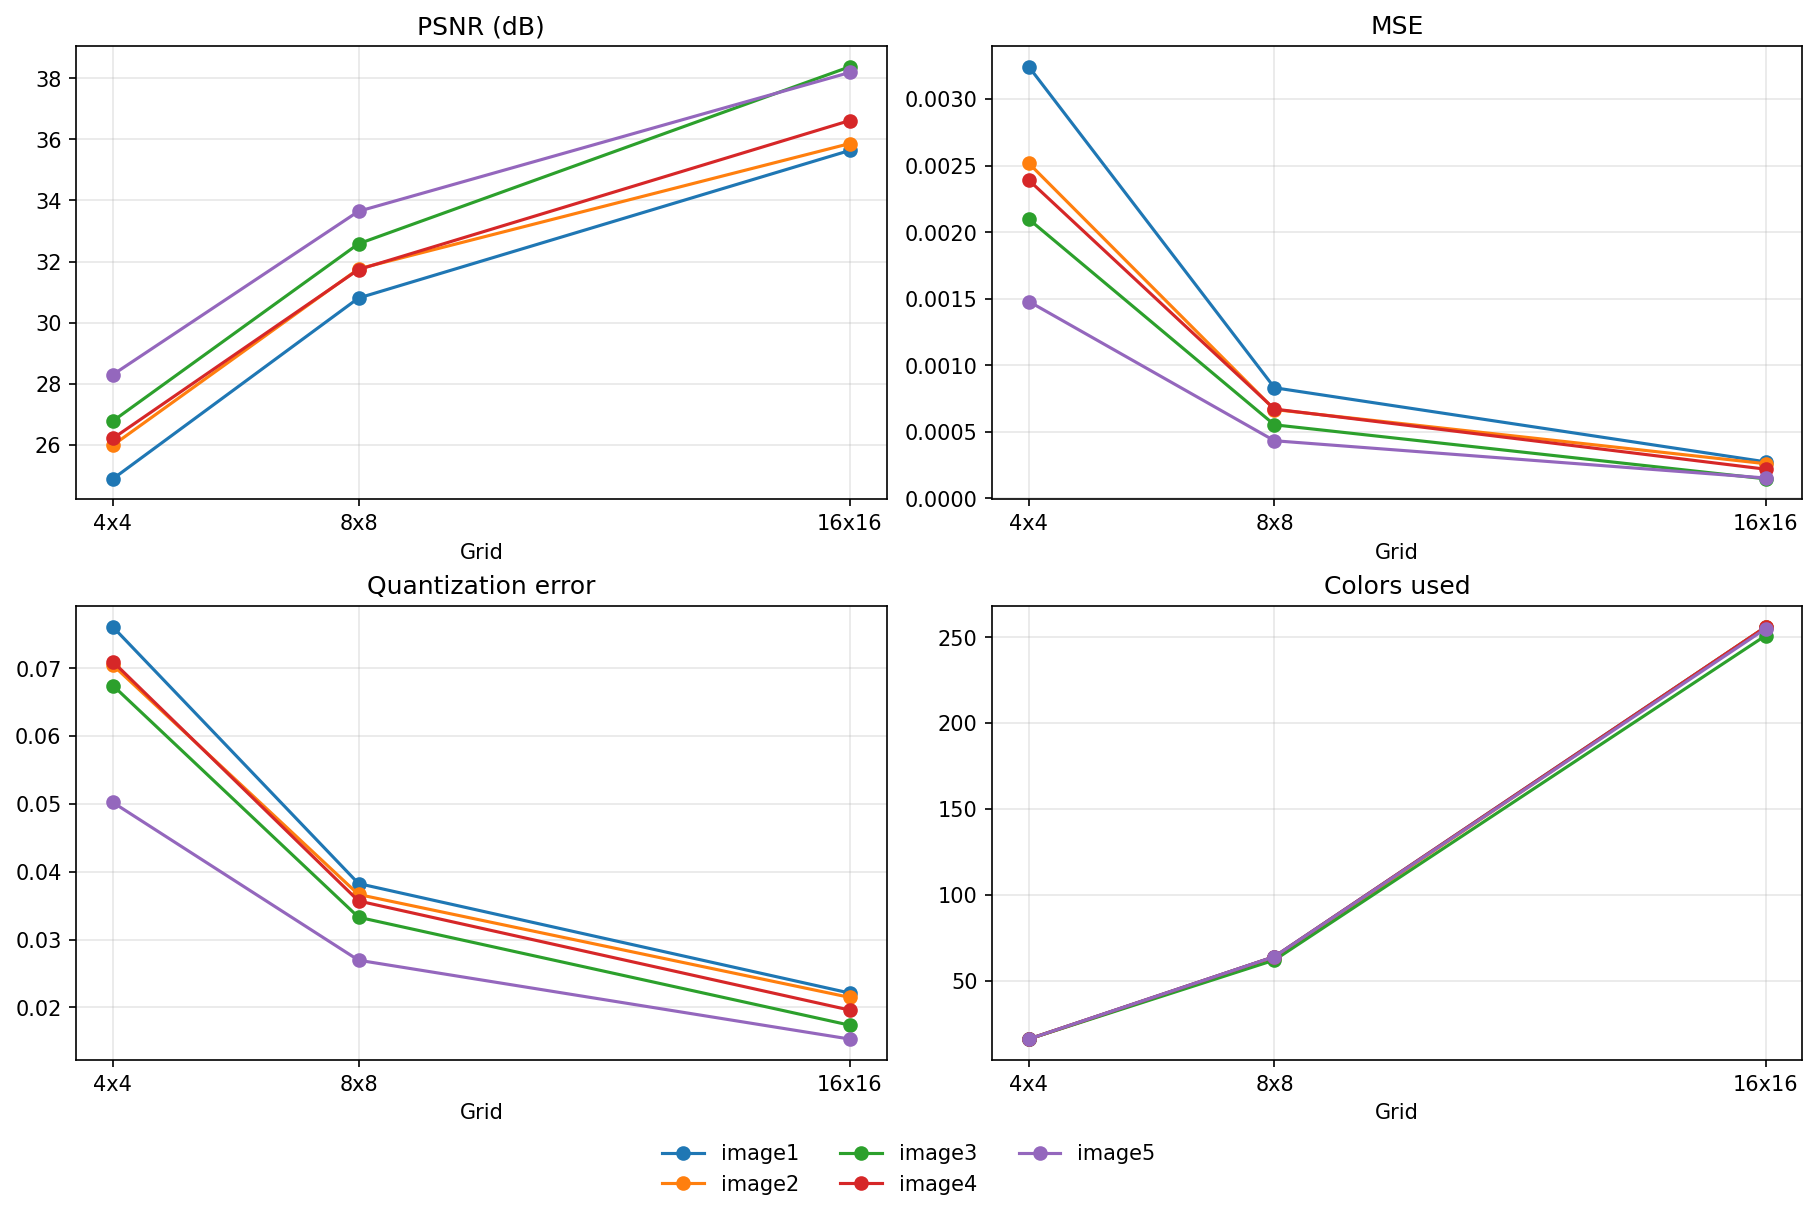
\includegraphics[width=\textwidth]{../som/results_som/metrics_comparison.png}
\caption{Curvas comparativas de desempenho da SOM (PSNR, MSE, erro de quantização e ocupação de cores) em função da dimensão da grade.}
\label{fig:som-metrics}
\end{figure}

\begin{figure}[H]
\centering
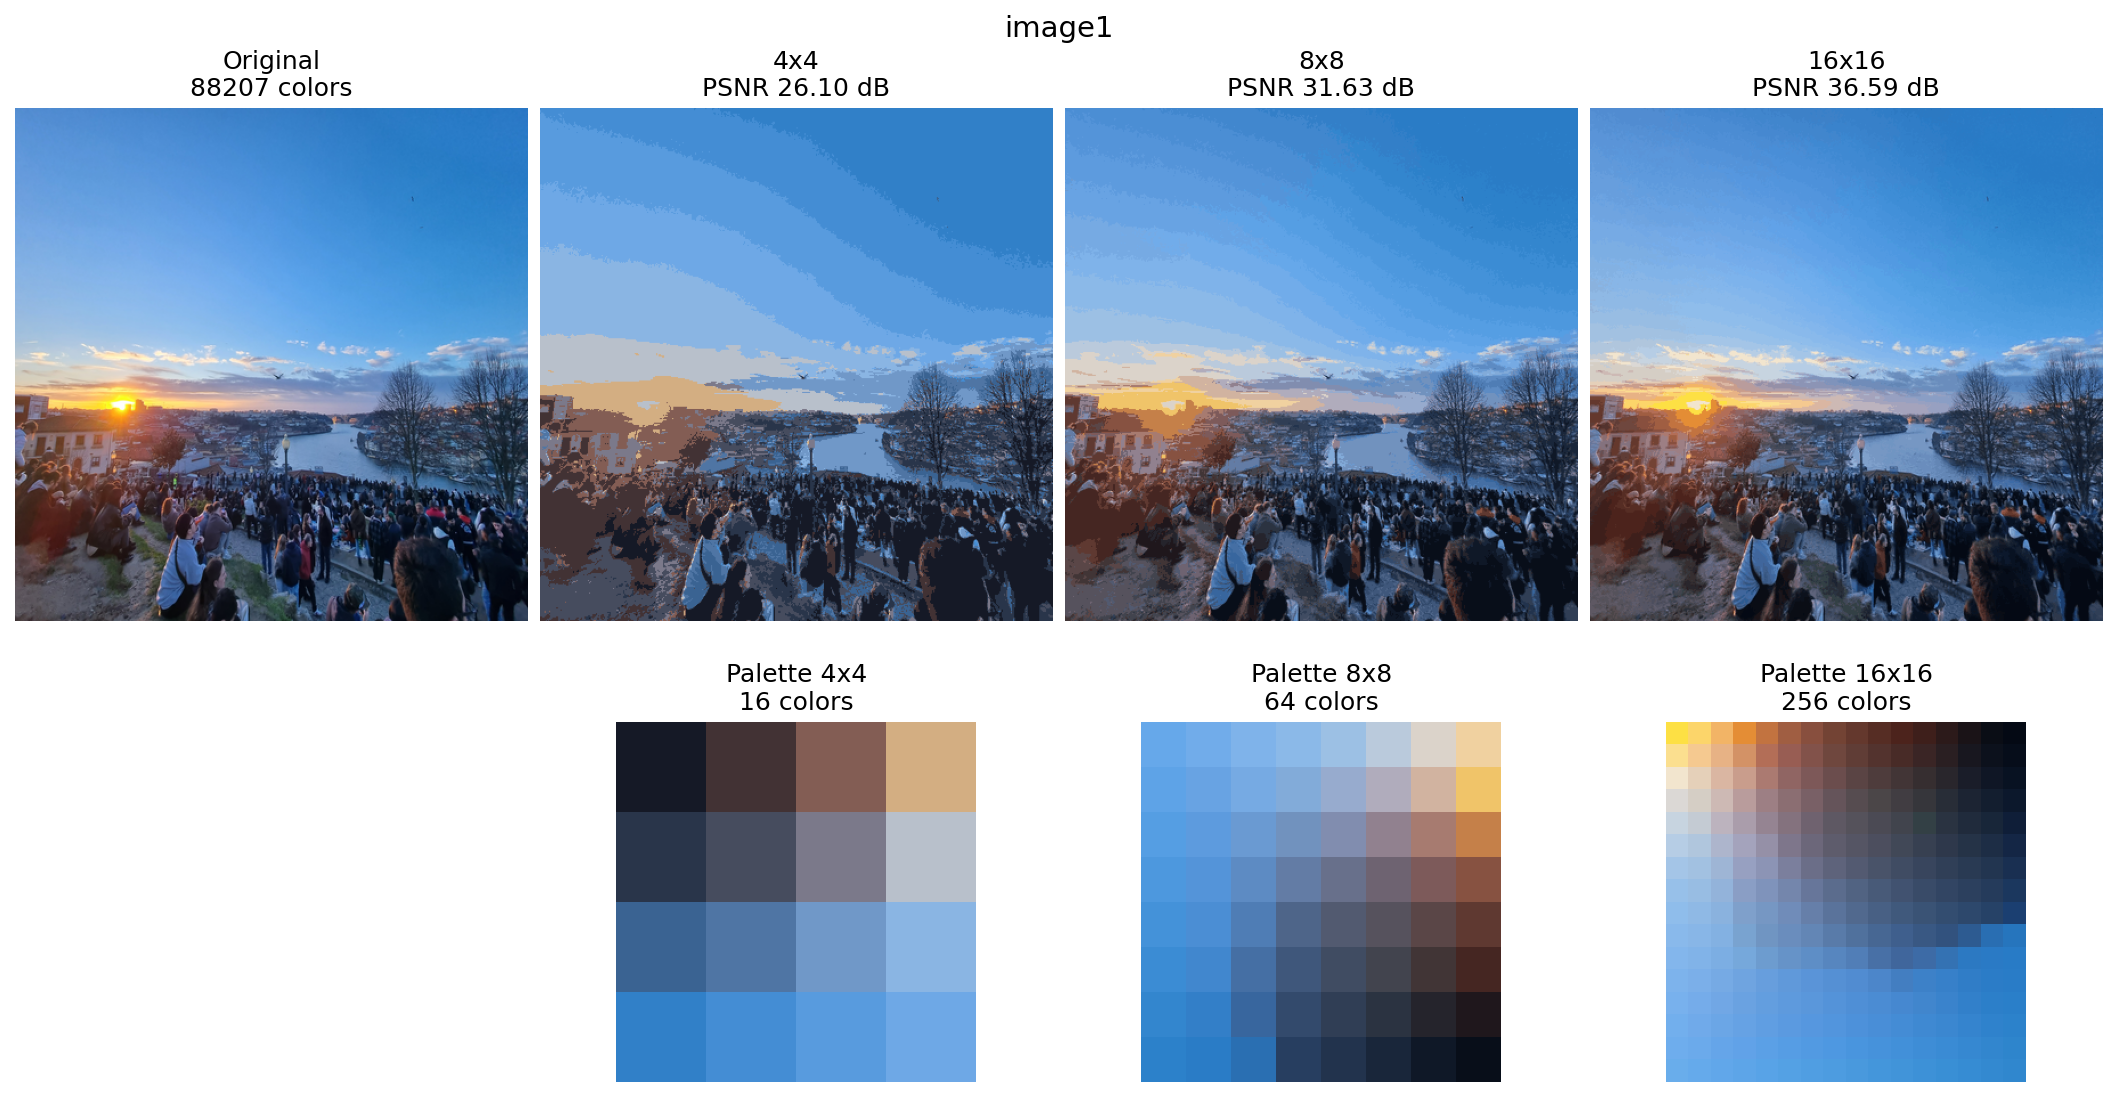
\includegraphics[width=\textwidth]{../som/results_som/image1.png}
\caption{Quantização por SOM em \texttt{image1} ($88\,207$ cores originais) sob as três configurações de grade, ressaltando o gradiente topológico da paleta resultante.}
\label{fig:som-1}
\end{figure}

\begin{figure}[H]
\centering
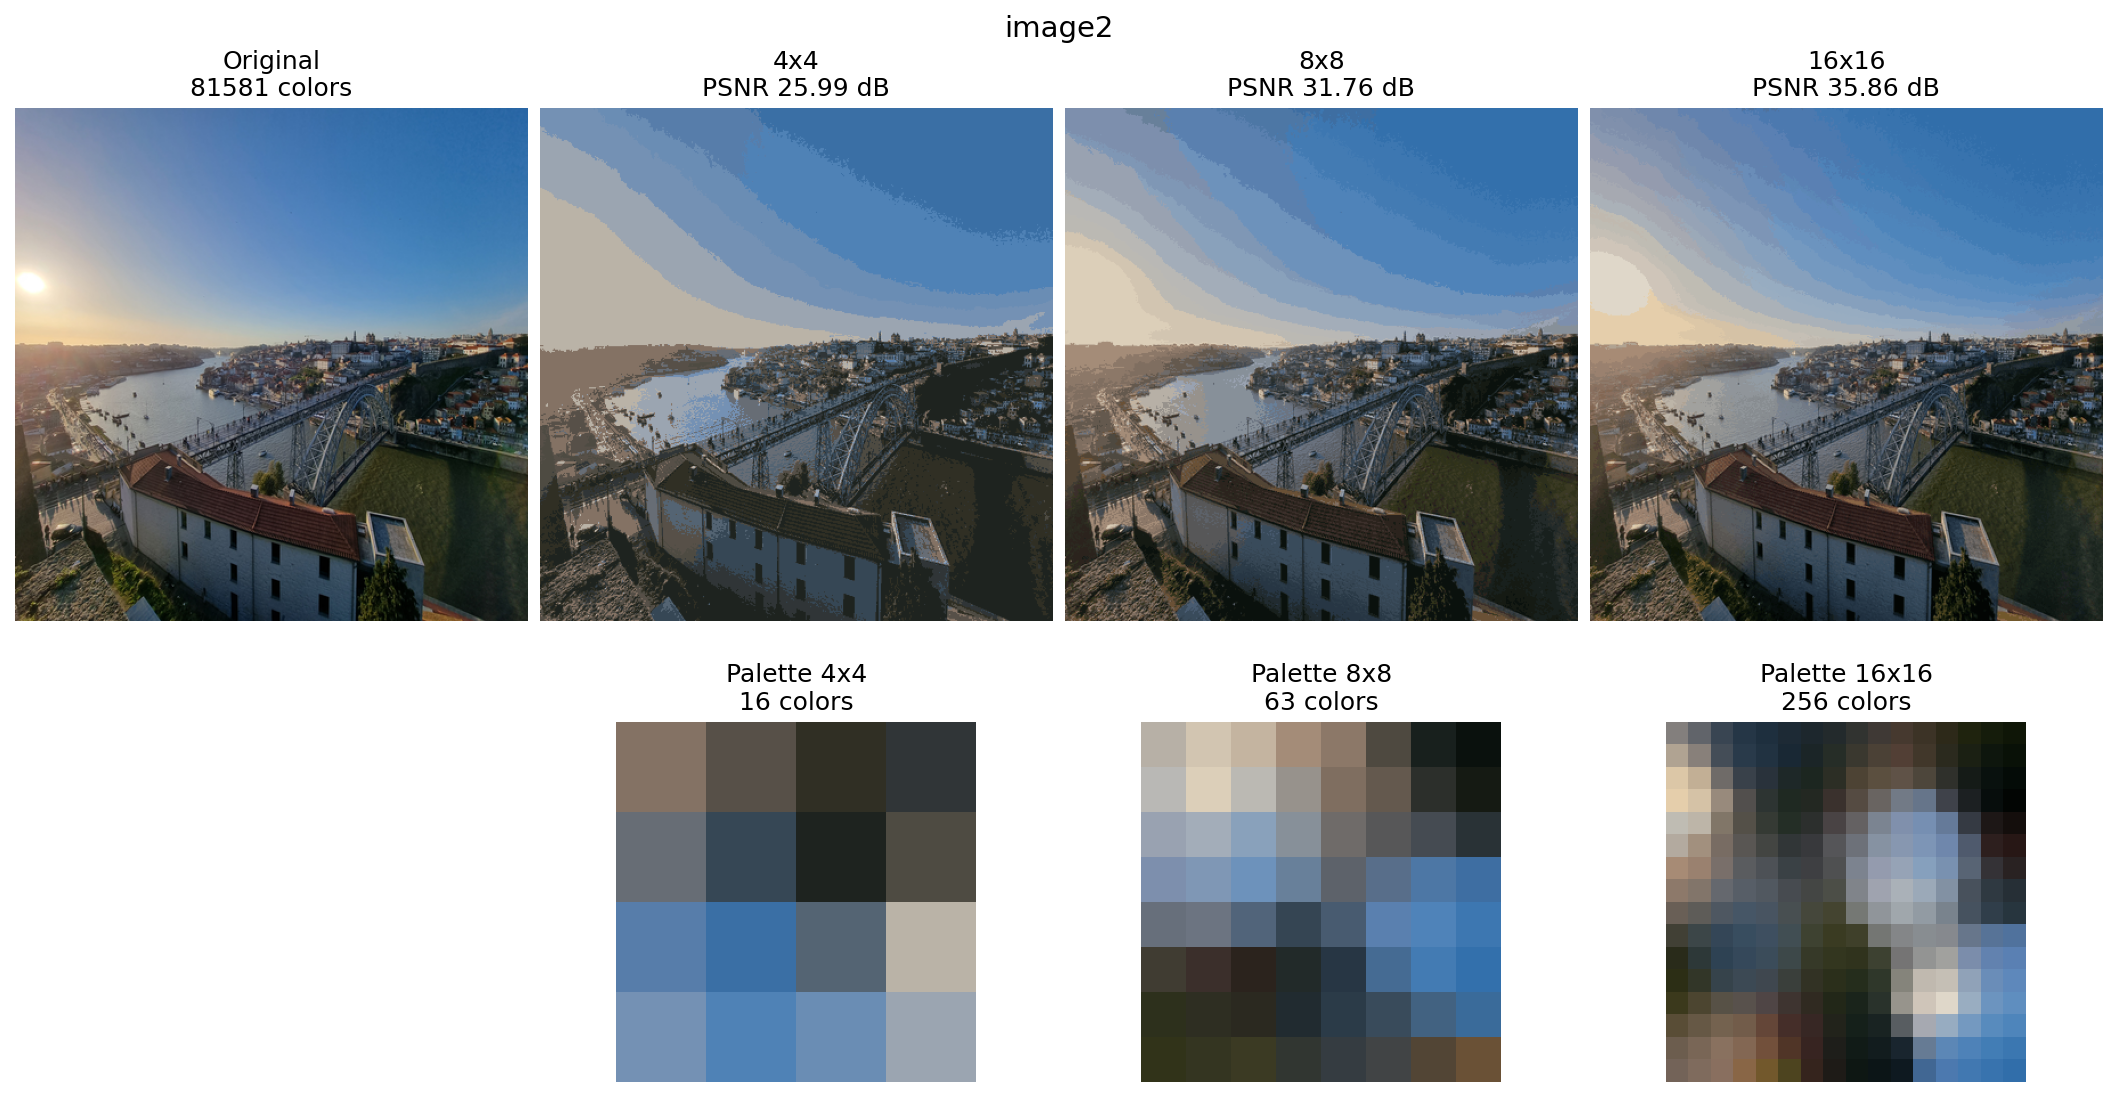
\includegraphics[width=\textwidth]{../som/results_som/image2.png}
\caption{Quantização por SOM em \texttt{image2}: organização contínua dos tons urbanos e aquáticos na grade $16 \times 16$.}
\label{fig:som-2}
\end{figure}

\begin{figure}[H]
\centering
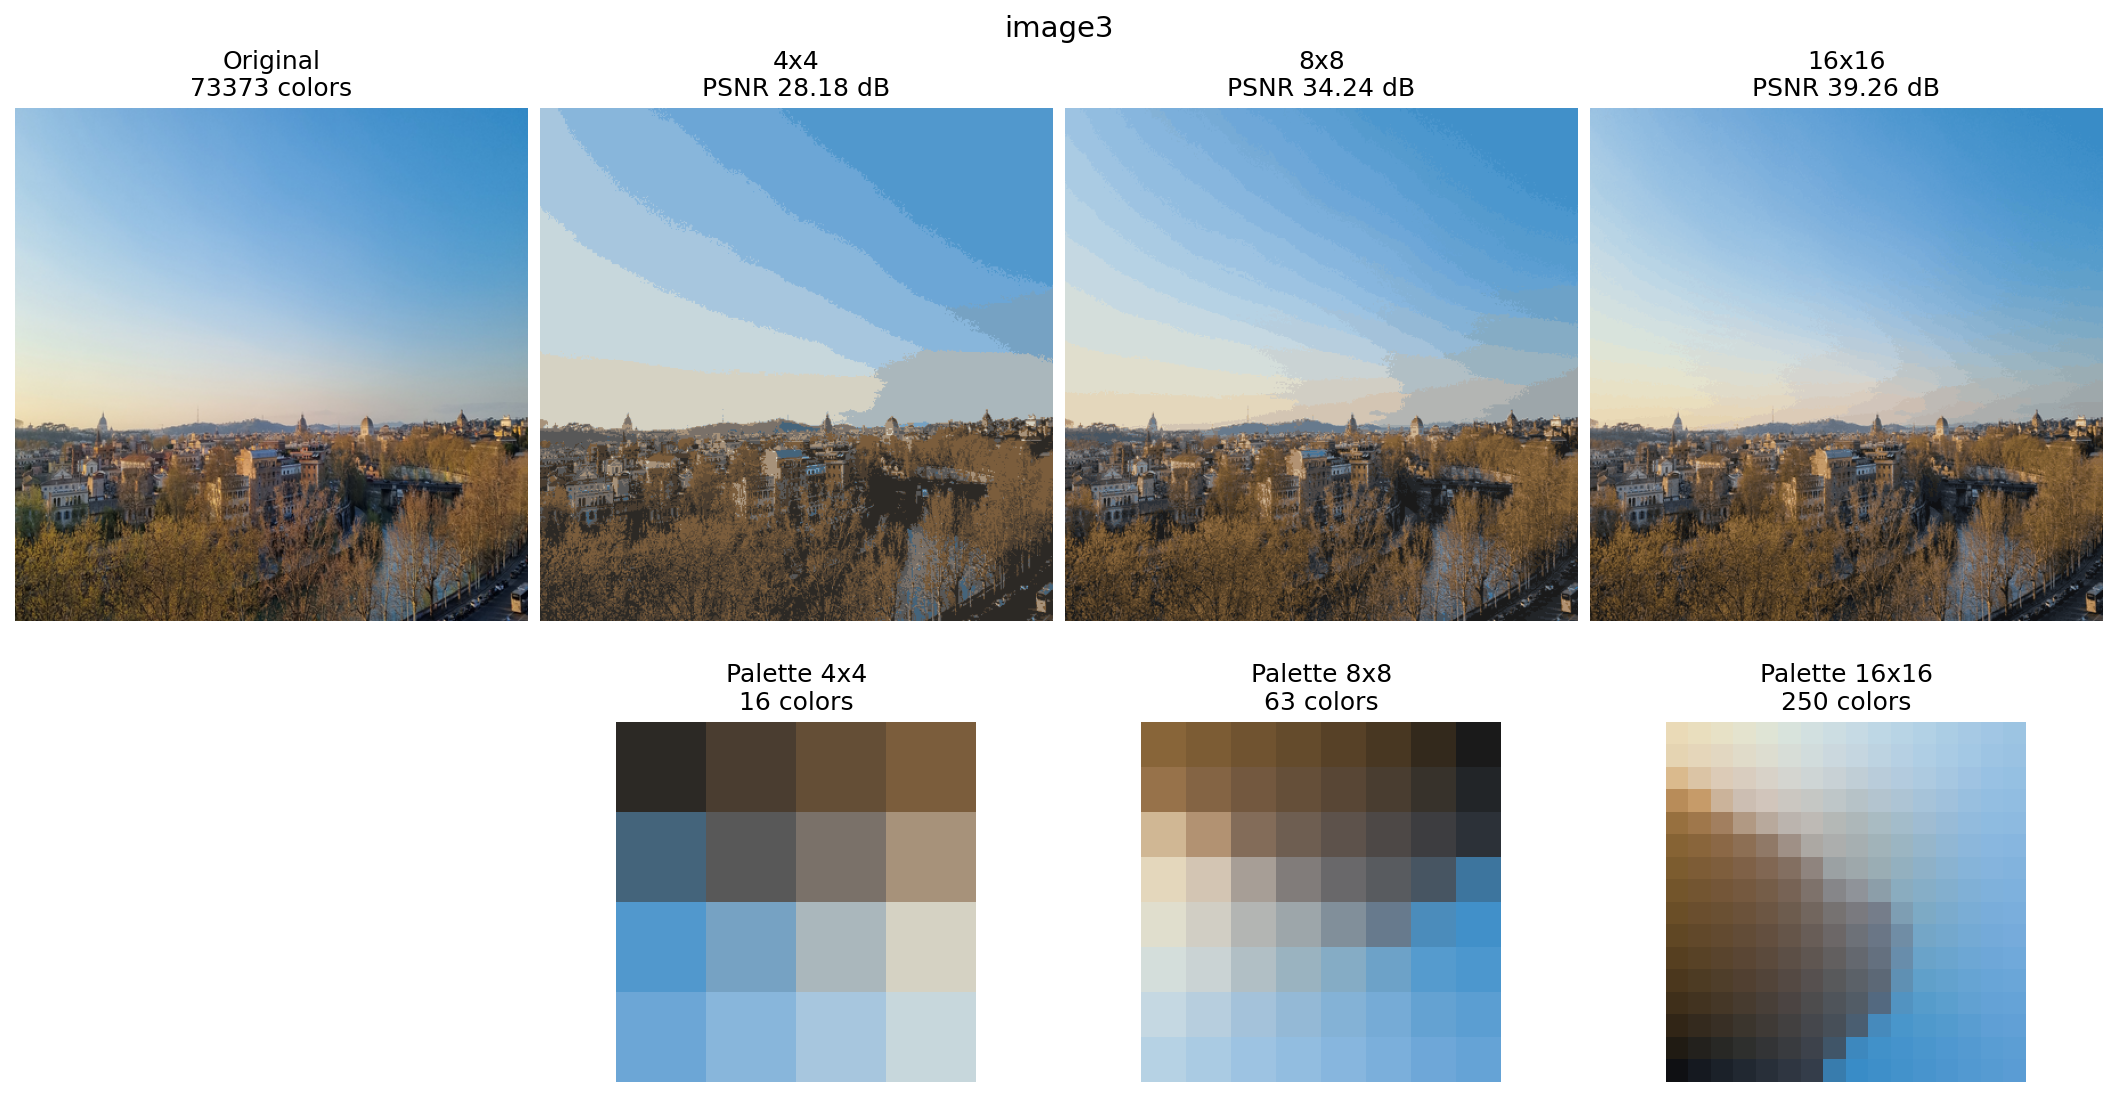
\includegraphics[width=\textwidth]{../som/results_som/image3.png}
\caption{Quantização por SOM em \texttt{image3}, configuração de maior PSNR entre as grades $16 \times 16$ ($39{,}26\,\mathrm{dB}$).}
\label{fig:som-3}
\end{figure}

\begin{figure}[H]
\centering
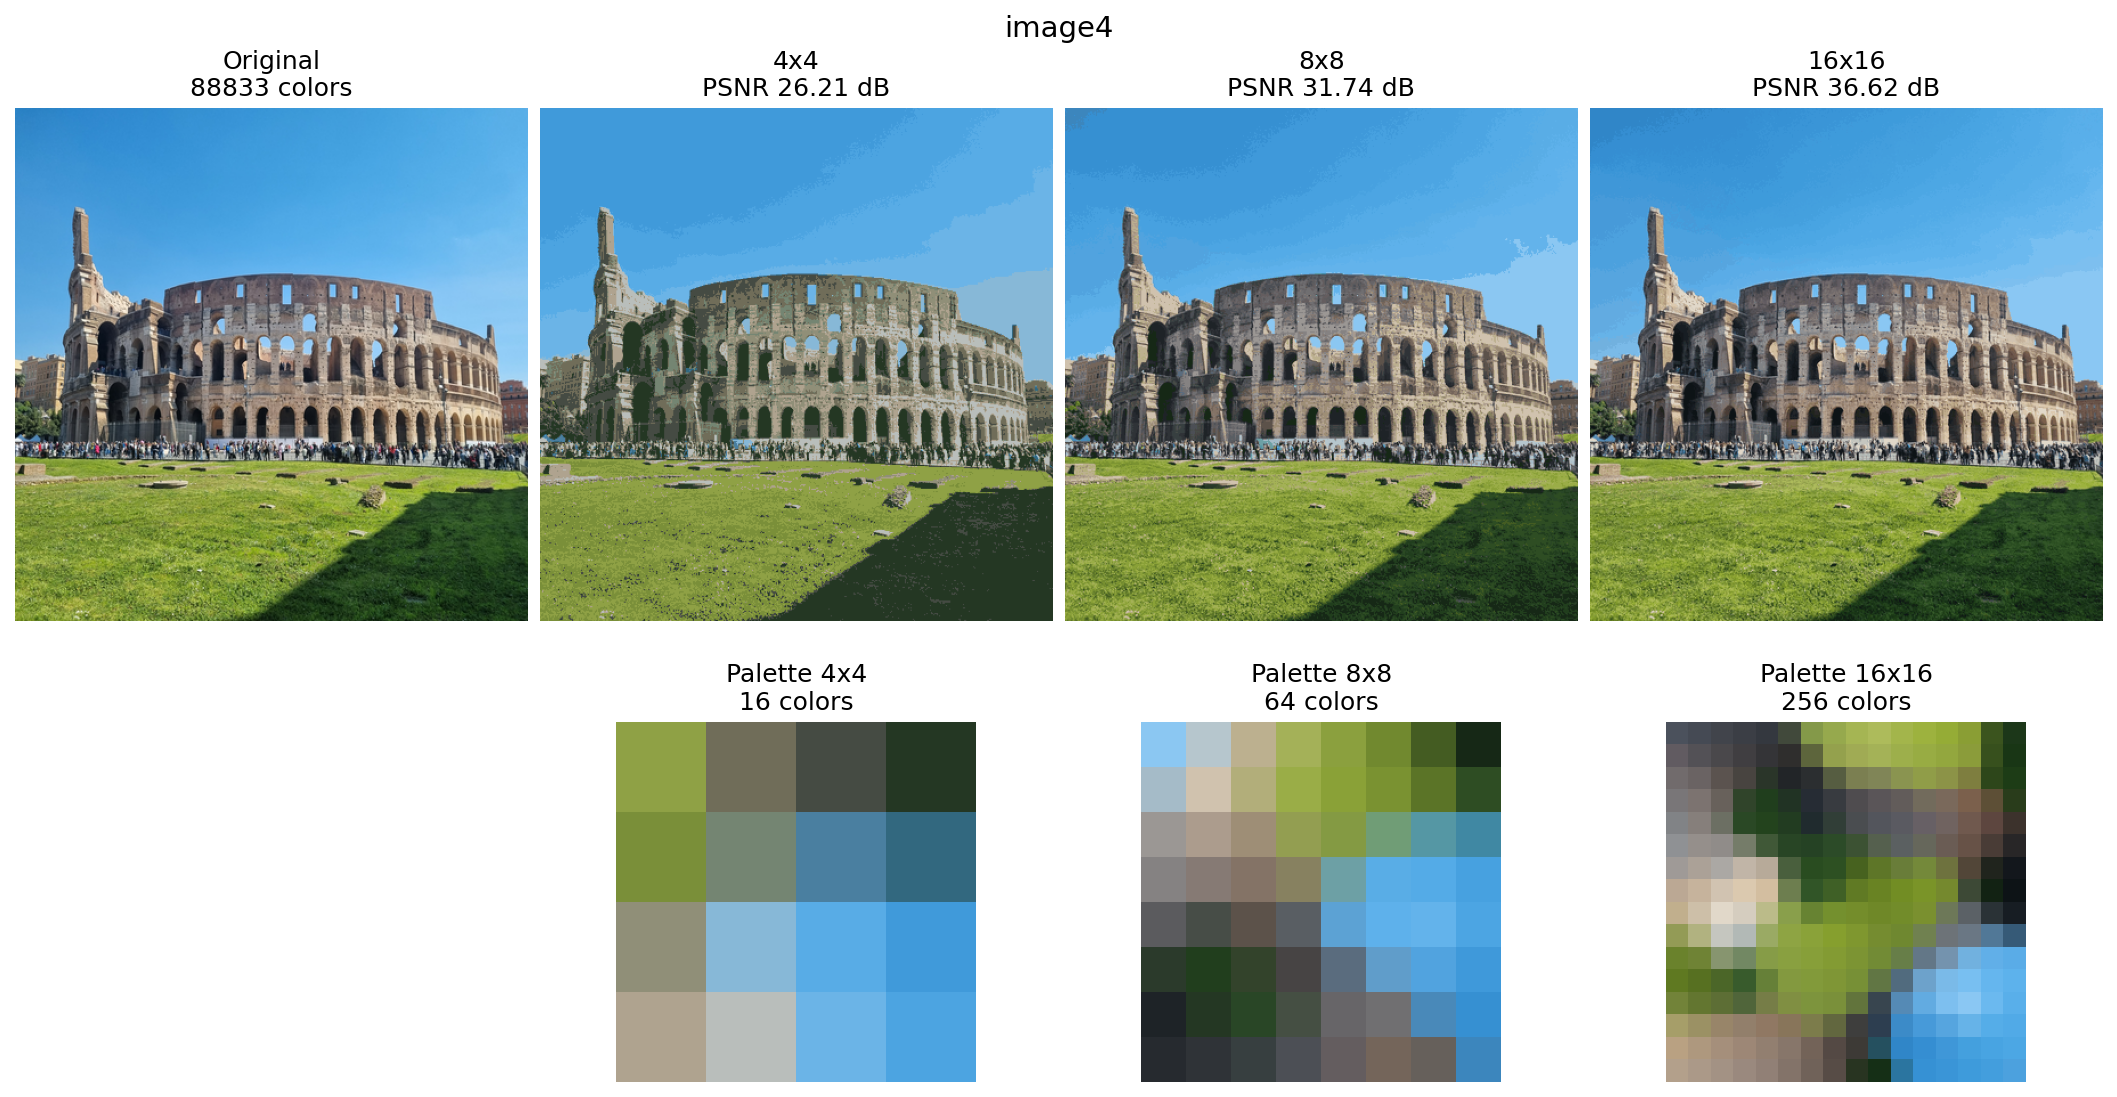
\includegraphics[width=\textwidth]{../som/results_som/image4.png}
\caption{Quantização por SOM em \texttt{image4}: separação contínua entre componentes de vegetação, alvenaria e céu.}
\label{fig:som-4}
\end{figure}

\begin{figure}[H]
\centering
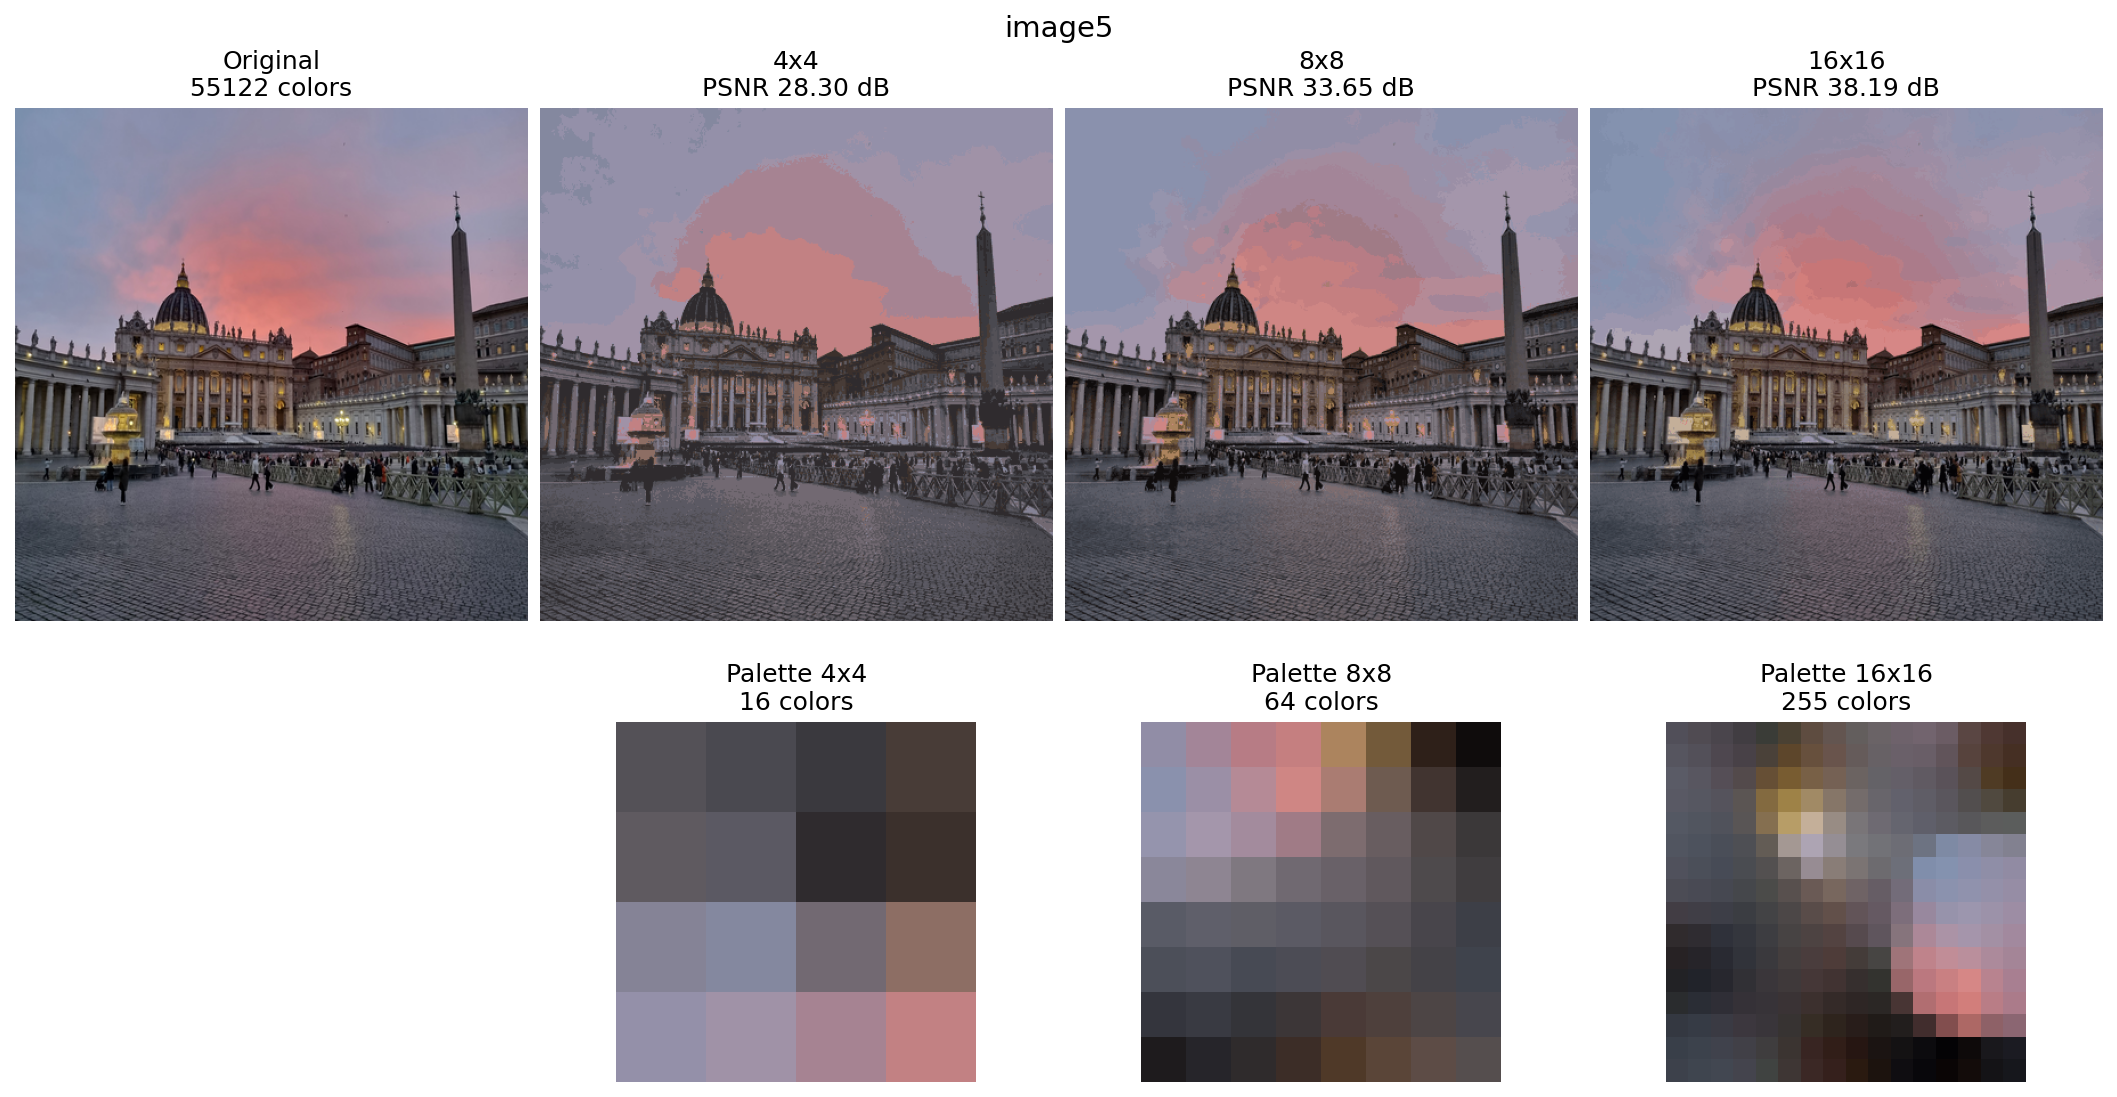
\includegraphics[width=\textwidth]{../som/results_som/image5.png}
\caption{Quantização por SOM em \texttt{image5}: transições entre zonas de sombra, matizes rosados e iluminação dourada.}
\label{fig:som-5}
\end{figure}

\section{Growing Neural Gas (GNG)}

Diferentemente da topologia fixa da SOM, o GNG constrói dinamicamente um grafo adaptativo não restrito a uma dimensão predefinida. O treinamento inicia-se com dois nós conectados aleatoriamente. Para cada vetor apresentado, o nó vencedor ($s_1$) e seus vizinhos topológicos são atualizados em direção à amostra, reforçando a aresta entre $s_1$ e o segundo protótipo mais próximo ($s_2$). Conexões com idade superior a $a_{\max}$ são sistematicamente eliminadas. Periodicamente, a cada $\lambda$ amostras, uma nova unidade é alocada entre o neurônio com maior erro acumulado e seu vizinho de maior discrepância.

O regime de treino foi executado ao longo de $5$ épocas sob amostragem aleatória ($1\,012\,500$ iterações). Os hiperparâmetros adotados constam na Tabela~\ref{tab:gng-hp}. Com $\lambda = 2000$, o processo de expansão até $256$ nós conclui-se em $508\,000$ iterações (aproximadamente $50\%$ do orçamento computacional total), reservando a metade restante exclusivamente para a estabilização e ajuste fino dos pesos sinápticos. A constante de decaimento de erro $\beta = 0{,}99975$ confere uma janela efetiva de memória de $1/(1-\beta) = 4000$ amostras, integrando o erro acumulado em um intervalo correspondente a duas inserções sucessivas ($2\lambda$).

\begin{table}[H]
\centering
\caption{Hiperparâmetros empregados no treinamento da rede GNG.}
\label{tab:gng-hp}
\begin{tabular}{lll}
\toprule
Parâmetro & Valor & Função Operacional \\
\midrule
$\varepsilon_b$ (\texttt{lr\_winner})   & $0{,}05$     & Taxa de aprendizado da unidade vencedora \\
$\varepsilon_n$ (\texttt{lr\_neighbor}) & $0{,}0006$   & Taxa de aprendizado dos vizinhos topológicos \\
$a_{\max}$ (\texttt{max\_edge\_age})    & $50$         & Limiar de idade para remoção de arestas \\
$\lambda$ (\texttt{lambda\_steps})      & $2000$       & Intervalo de amostragem entre inserções neurais \\
$\alpha$                                & $0{,}5$      & Fator de atenuação do erro local na inserção \\
$\beta$                                 & $0{,}99975$  & Taxa de decaimento do erro a cada iteração \\
Épocas                                  & $5$          & Passagens iterativas sobre o conjunto de pixels \\
\bottomrule
\end{tabular}
\end{table}

\begin{table}[H]
\centering
\caption{Métricas obtidas com o modelo GNG após quantização para $8$ bits.}
\label{tab:gng}
\small
\begin{tabular}{llrrrr}
\toprule
Imagem & Neurônios & Erro de Quant. & MSE & PSNR (dB) & Cores Efetivas \\
\midrule
image1 & 16  & 0,0636 & $1{,}92 \times 10^{-3}$ & 27,16 & 16 \\
image1 & 64  & 0,0322 & $4{,}86 \times 10^{-4}$ & 33,14 & 64 \\
image1 & 256 & 0,0185 & $1{,}53 \times 10^{-4}$ & 38,16 & 256 \\
\midrule
image2 & 16  & 0,0550 & $1{,}30 \times 10^{-3}$ & 28,85 & 16 \\
image2 & 64  & 0,0286 & $3{,}39 \times 10^{-4}$ & 34,70 & 64 \\
image2 & 256 & 0,0161 & $1{,}08 \times 10^{-4}$ & 39,68 & 256 \\
\midrule
image3 & 16  & 0,0518 & $1{,}21 \times 10^{-3}$ & 29,17 & 16 \\
image3 & 64  & 0,0262 & $3{,}03 \times 10^{-4}$ & 35,19 & 64 \\
image3 & 256 & 0,0147 & $9{,}36 \times 10^{-5}$ & 40,29 & 256 \\
\midrule
image4 & 16  & 0,0541 & $1{,}34 \times 10^{-3}$ & 28,72 & 16 \\
image4 & 64  & 0,0289 & $3{,}86 \times 10^{-4}$ & 34,13 & 64 \\
image4 & 256 & 0,0170 & $1{,}34 \times 10^{-4}$ & 38,73 & 252 \\
\midrule
image5 & 16  & 0,0399 & $7{,}65 \times 10^{-4}$ & 31,16 & 16 \\
image5 & 64  & 0,0214 & $2{,}15 \times 10^{-4}$ & 36,68 & 64 \\
image5 & 256 & 0,0126 & $7{,}28 \times 10^{-5}$ & 41,38 & 255 \\
\midrule
Média  & 16  & 0,0529 & $1{,}31 \times 10^{-3}$ & 29,01 & 16,0 \\
Média  & 64  & 0,0275 & $3{,}46 \times 10^{-4}$ & 34,77 & 64,0 \\
Média  & 256 & 0,0158 & $1{,}12 \times 10^{-4}$ & 39,65 & 255,0 \\
\bottomrule
\end{tabular}
\end{table}

O PSNR médio do GNG evoluiu de $29{,}01\,\mathrm{dB}$ ($16$ neurônios) para $34{,}77\,\mathrm{dB}$ ($64$ neurônios) e $39{,}65\,\mathrm{dB}$ ($256$ neurônios). O aproveitamento do codebook foi praticamente integral: com $16$ e $64$ unidades, não houve sobreposição cromática; no limite de $256$ neurônios, registraram-se apenas perdas residuais em \texttt{image4} ($252$ cores) e \texttt{image5} ($255$ cores). A inserção guiada por densidade e acúmulo de erro evita a concentração excessiva de nós em volumes restritos.

Ao analisar a representação visual da paleta em mosaico, nota-se ausência de ordenamento bidimensional aparente, uma vez que os nós são indexados conforme a ordem de alocação temporal e não projetados em um reticulado euclidiano regular. Contudo, a estrutura intrínseca revela-se quando o próprio grafo é inspecionado (Figura~\ref{fig:gng-graph}): ao projetar os pesos de \texttt{image5} via PCA, constata-se que os dois primeiros componentes principais retêm $98{,}6\%$ da variância total ($92{,}0\%$ em PC1 e $6{,}6\%$ em PC2). O grafo mapeia a variedade dimensional subjacente de forma coesa, estendendo-se do espectro escuro até os tons quentes de forma contínua, sem conexões espúrias entre extremos cromáticos.

\begin{figure}[H]
\centering
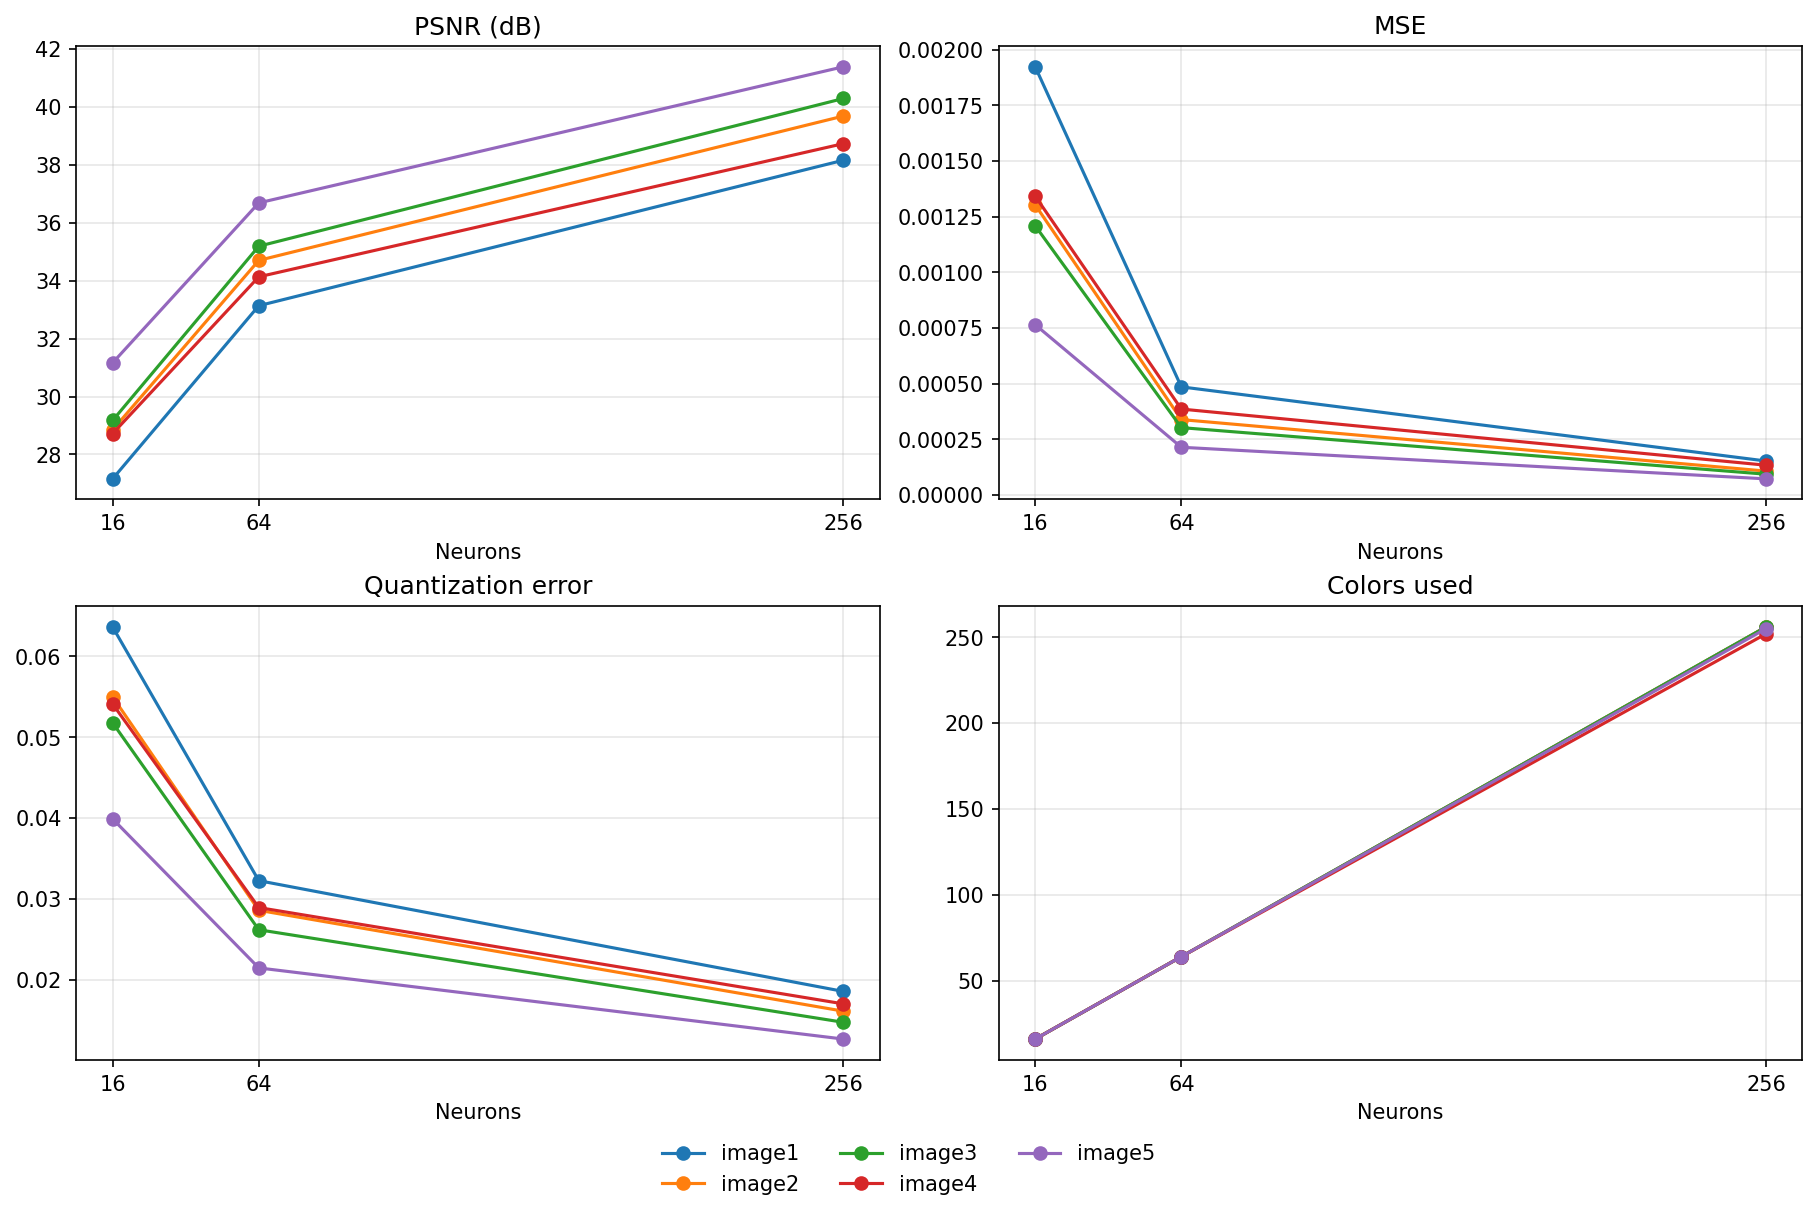
\includegraphics[width=\textwidth]{../gng/results_gng/metrics_comparison.png}
\caption{Evolução do desempenho do GNG em função da capacidade do modelo.}
\label{fig:gng-metrics}
\end{figure}

\begin{figure}[H]
\centering
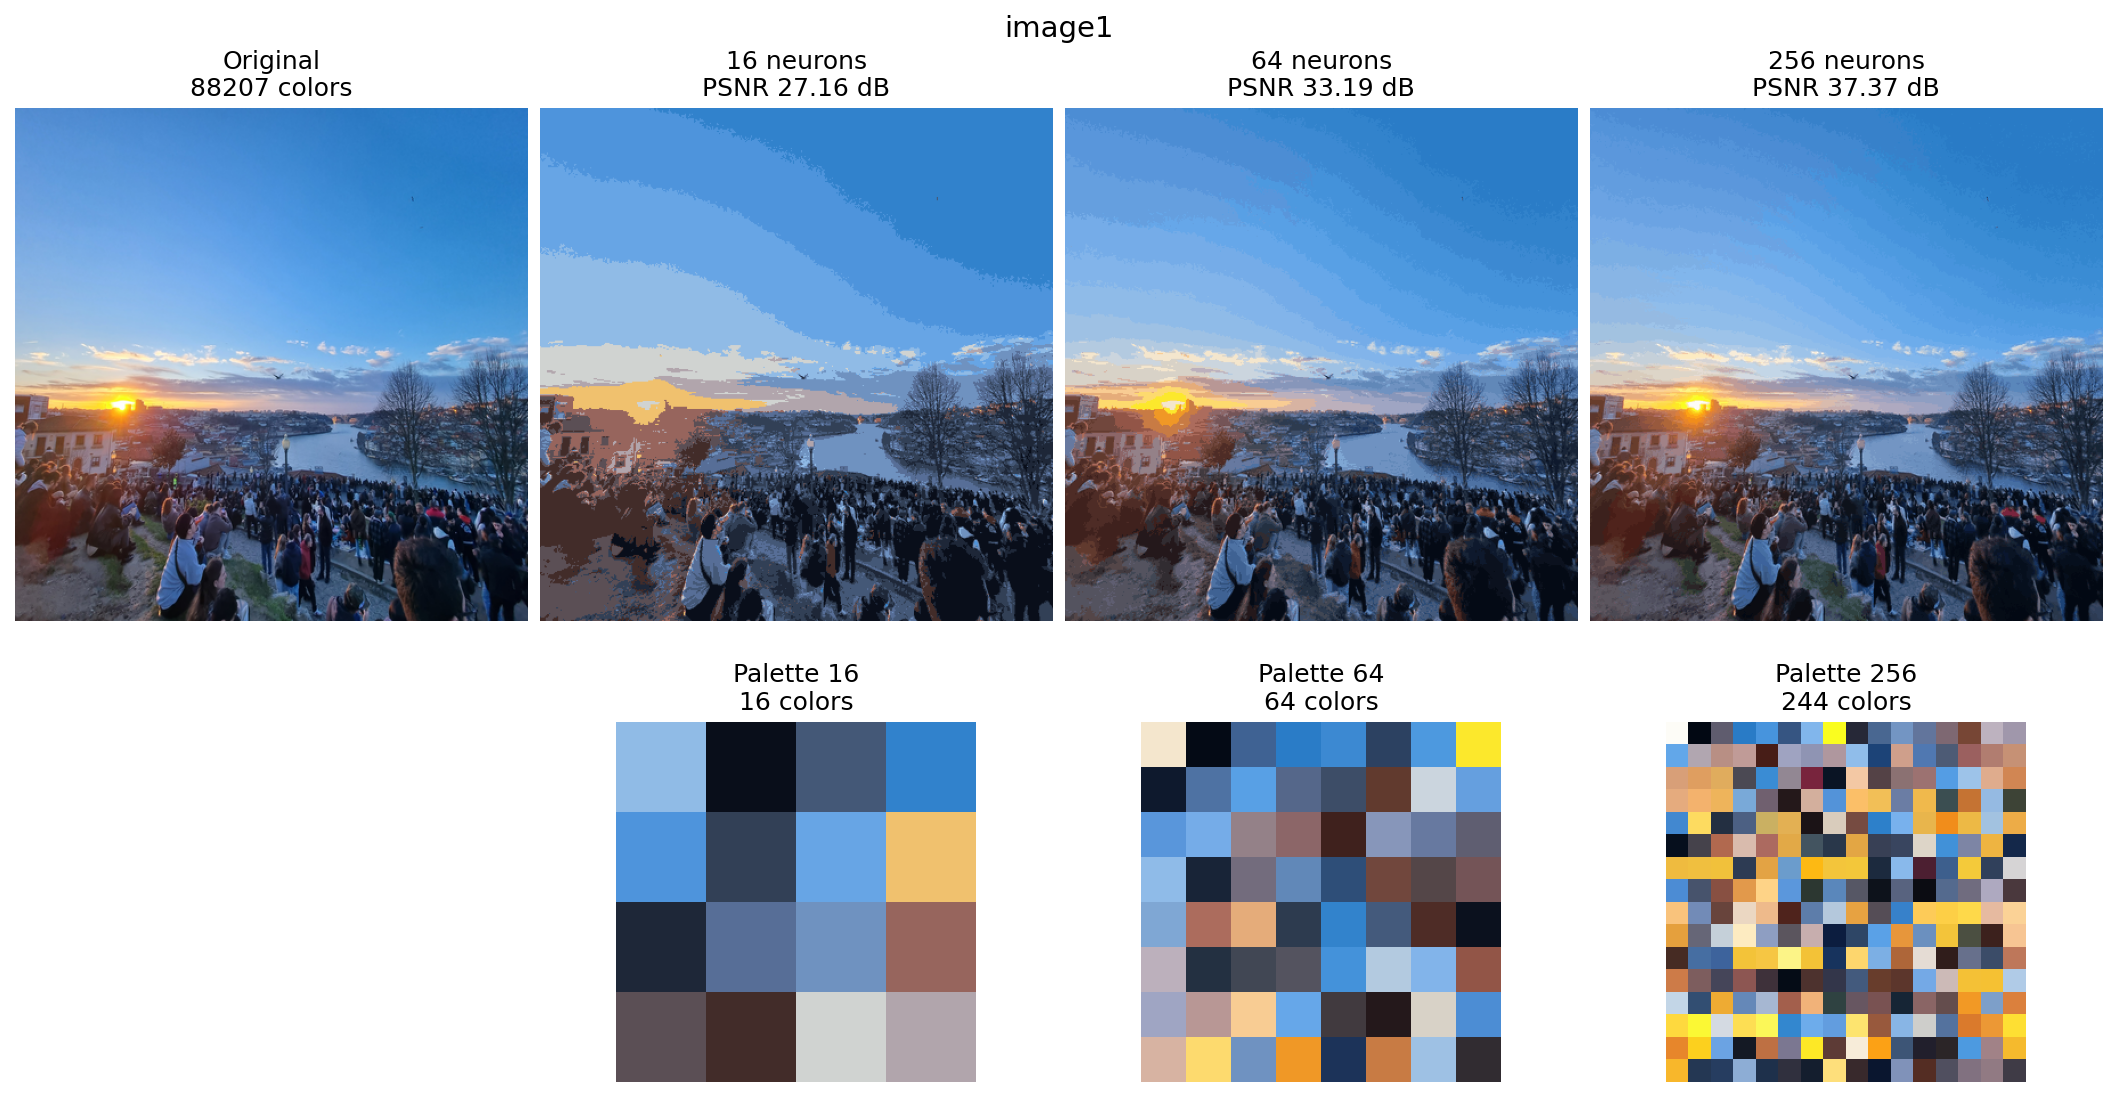
\includegraphics[width=\textwidth]{../gng/results_gng/image1.png}
\caption{Quantização por GNG em \texttt{image1}: preservação de componentes cromáticas minoritárias de alta saturação (e.g., o centro do sol) desde $16$ protótipos.}
\label{fig:gng-1}
\end{figure}

\begin{figure}[H]
\centering
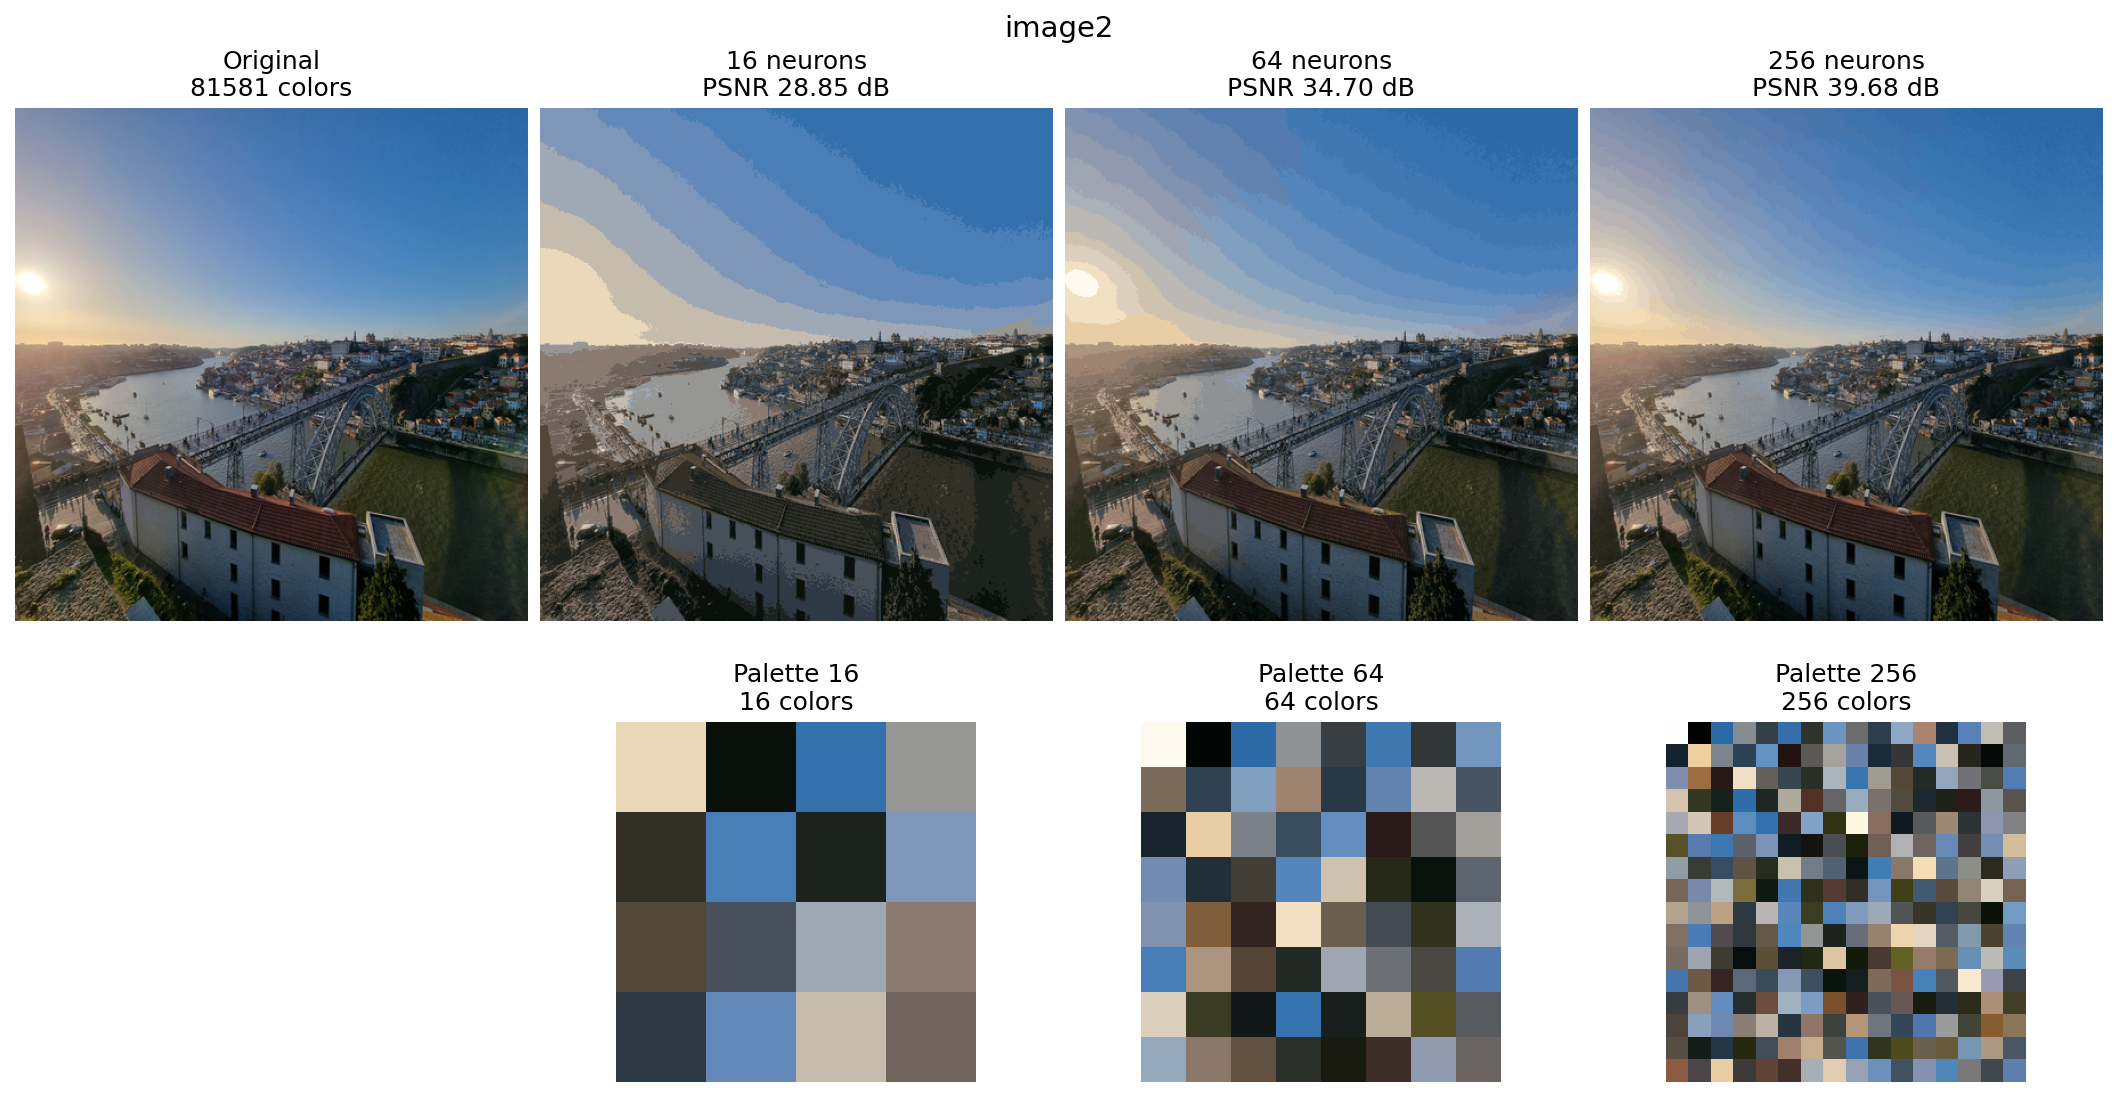
\includegraphics[width=\textwidth]{../gng/results_gng/image2.png}
\caption{Reconstruções via GNG em \texttt{image2}.}
\label{fig:gng-2}
\end{figure}

\begin{figure}[H]
\centering
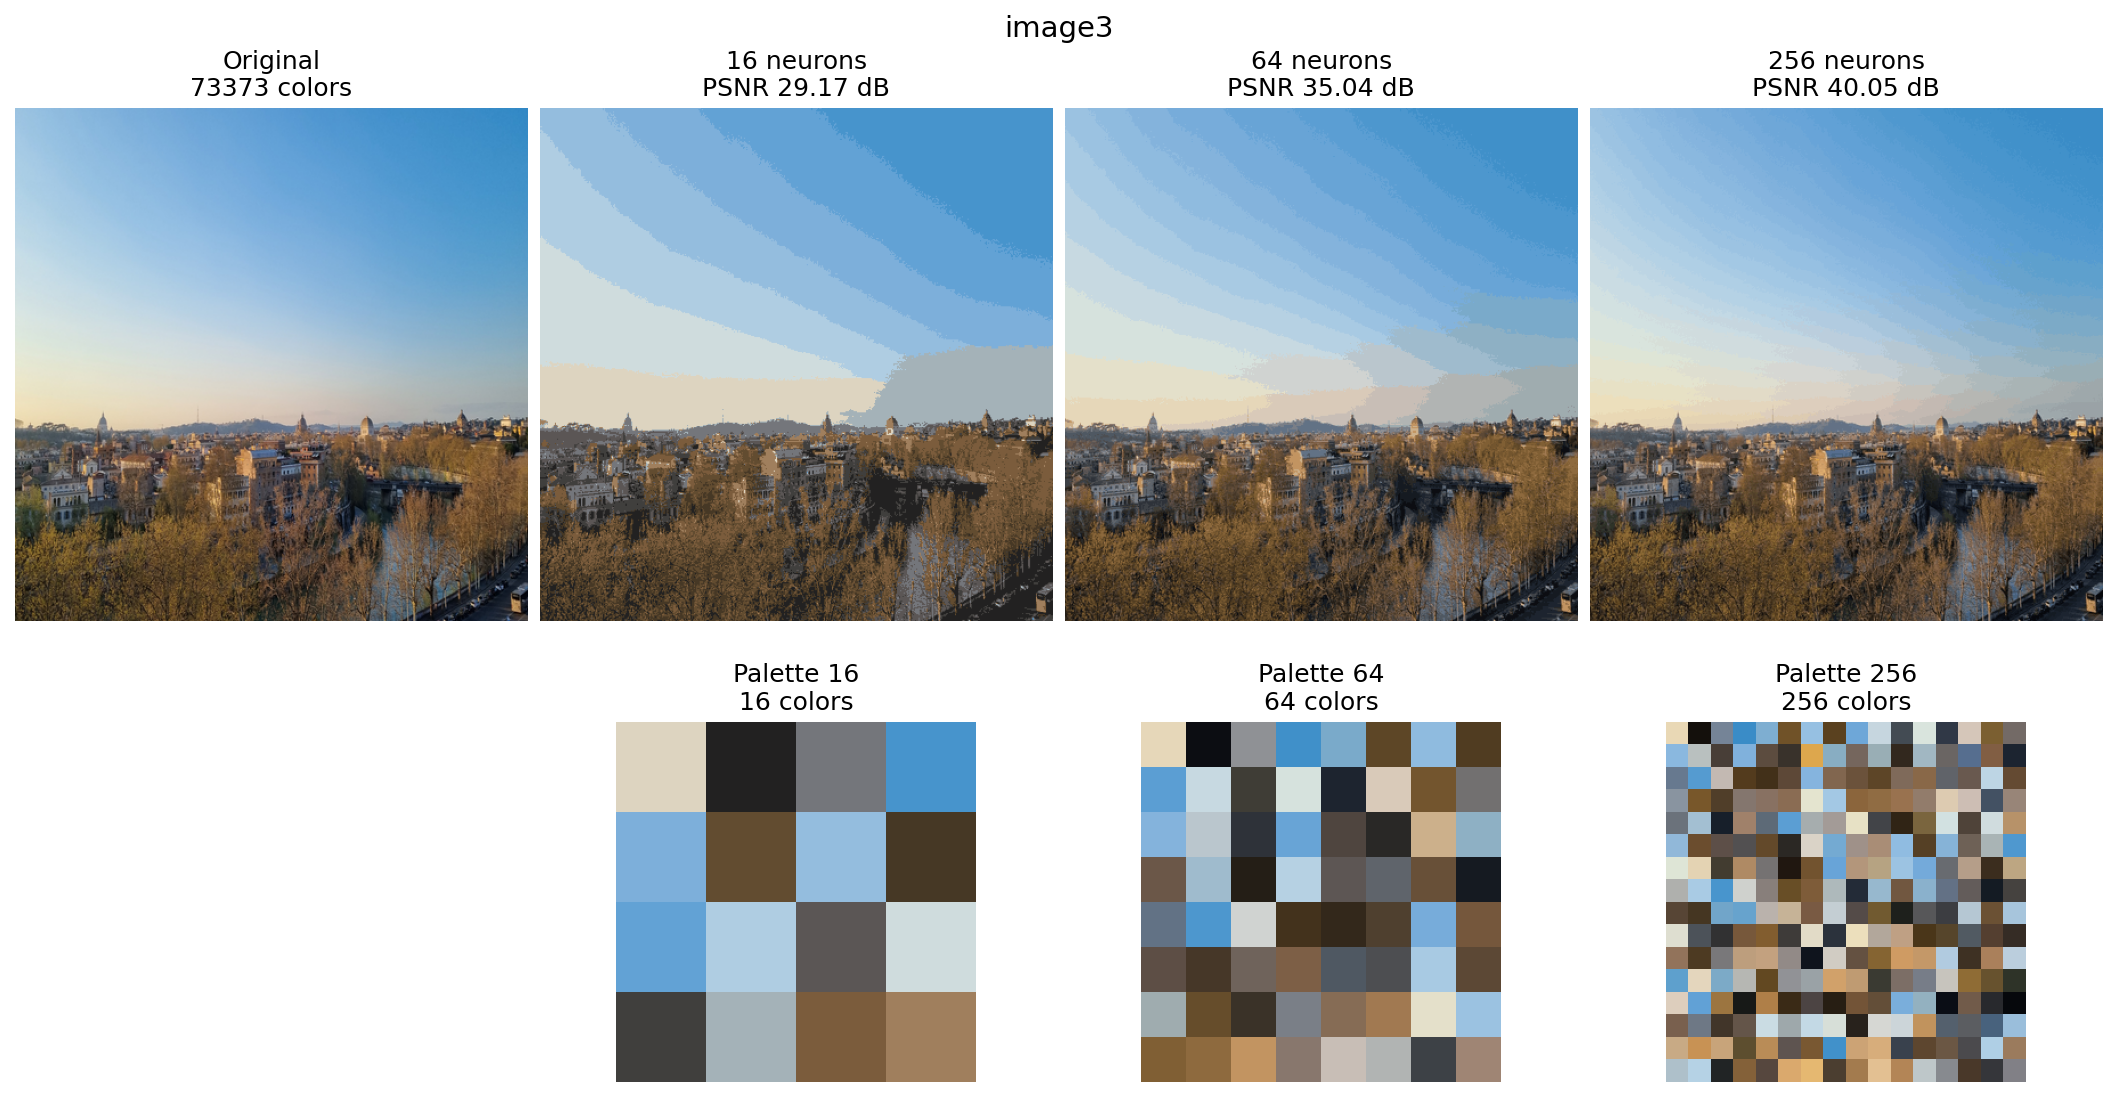
\includegraphics[width=\textwidth]{../gng/results_gng/image3.png}
\caption{Reconstruções via GNG em \texttt{image3}, superando a marca de $40\,\mathrm{dB}$ de PSNR com $256$ unidades.}
\label{fig:gng-3}
\end{figure}

\begin{figure}[H]
\centering
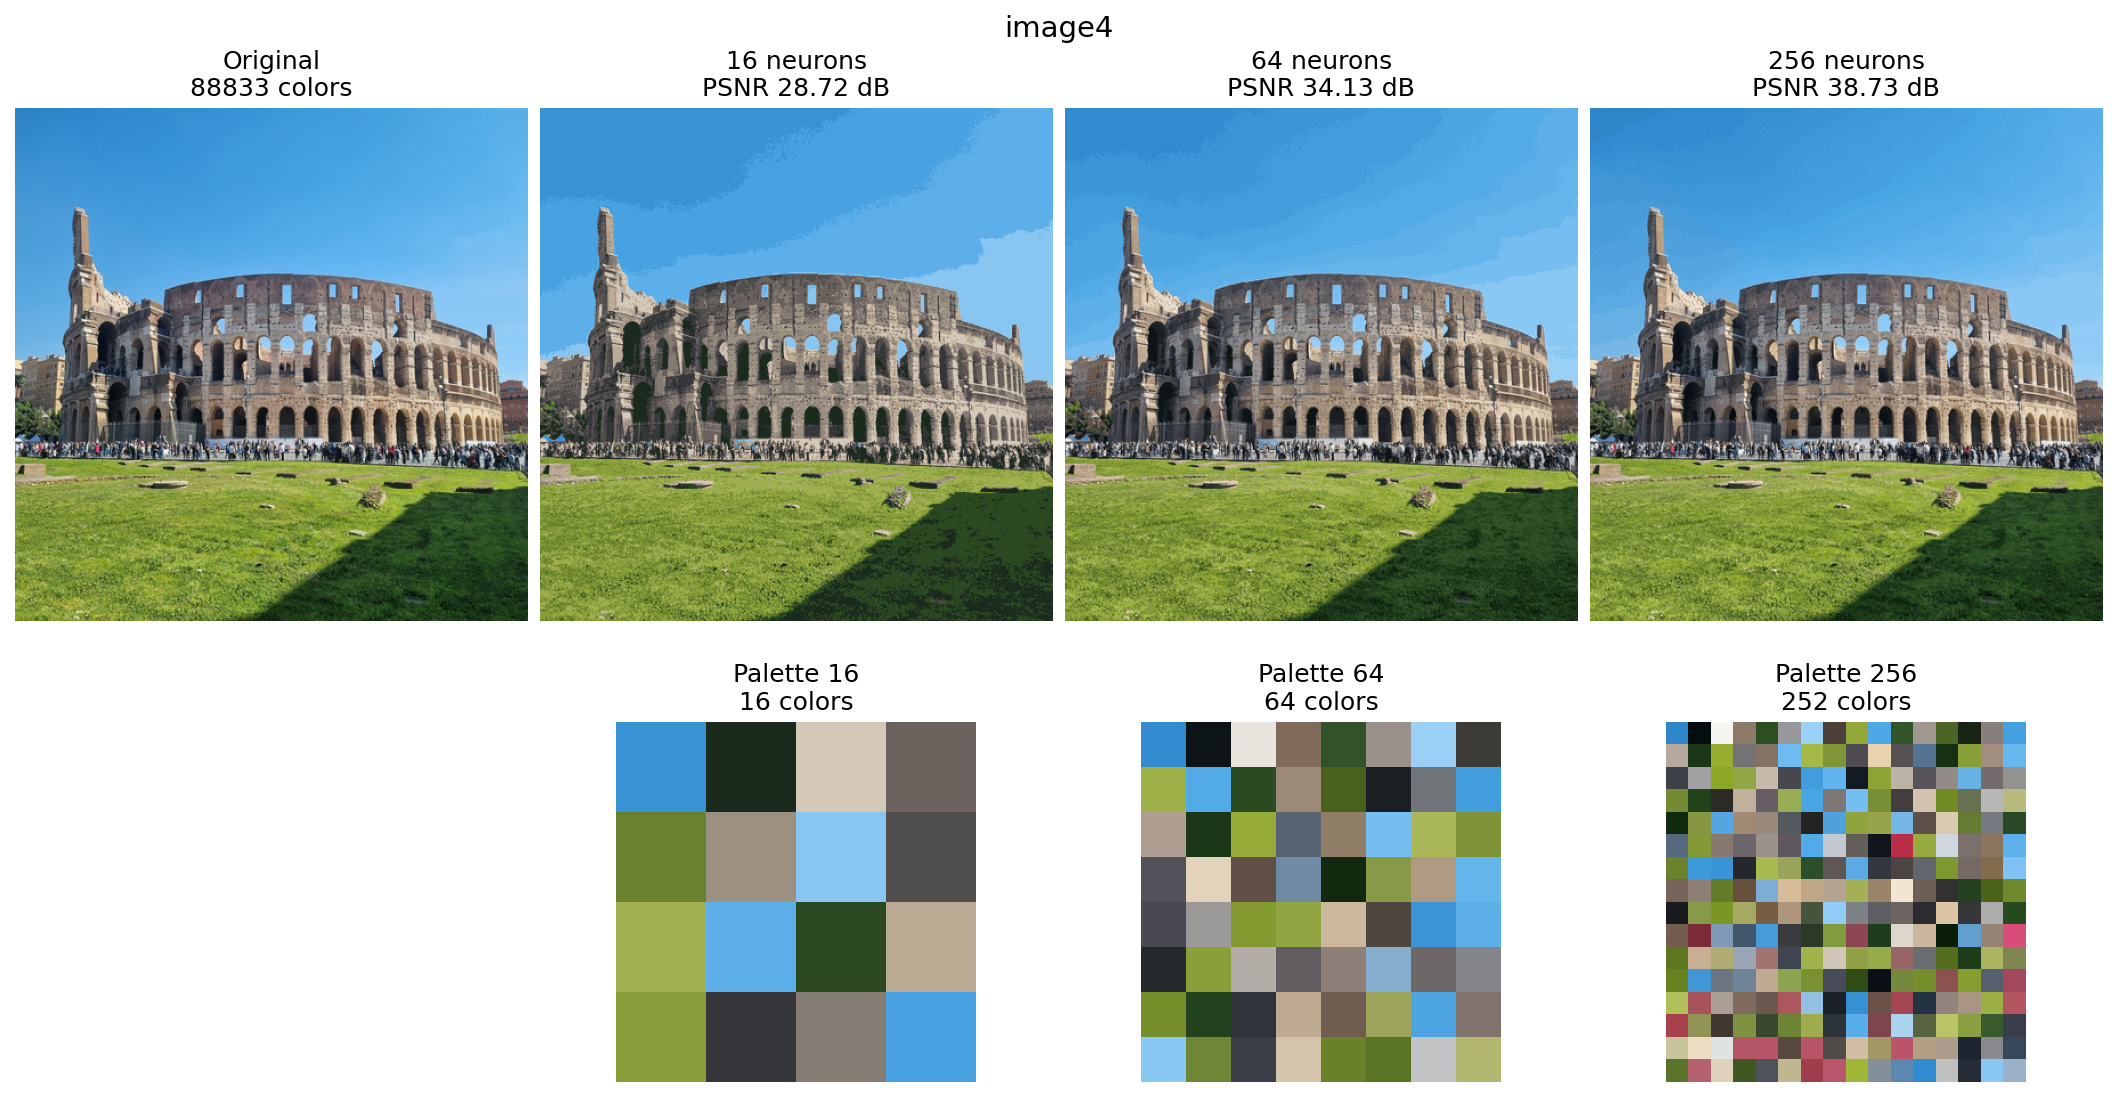
\includegraphics[width=\textwidth]{../gng/results_gng/image4.png}
\caption{Reconstruções via GNG em \texttt{image4}.}
\label{fig:gng-4}
\end{figure}

\begin{figure}[H]
\centering
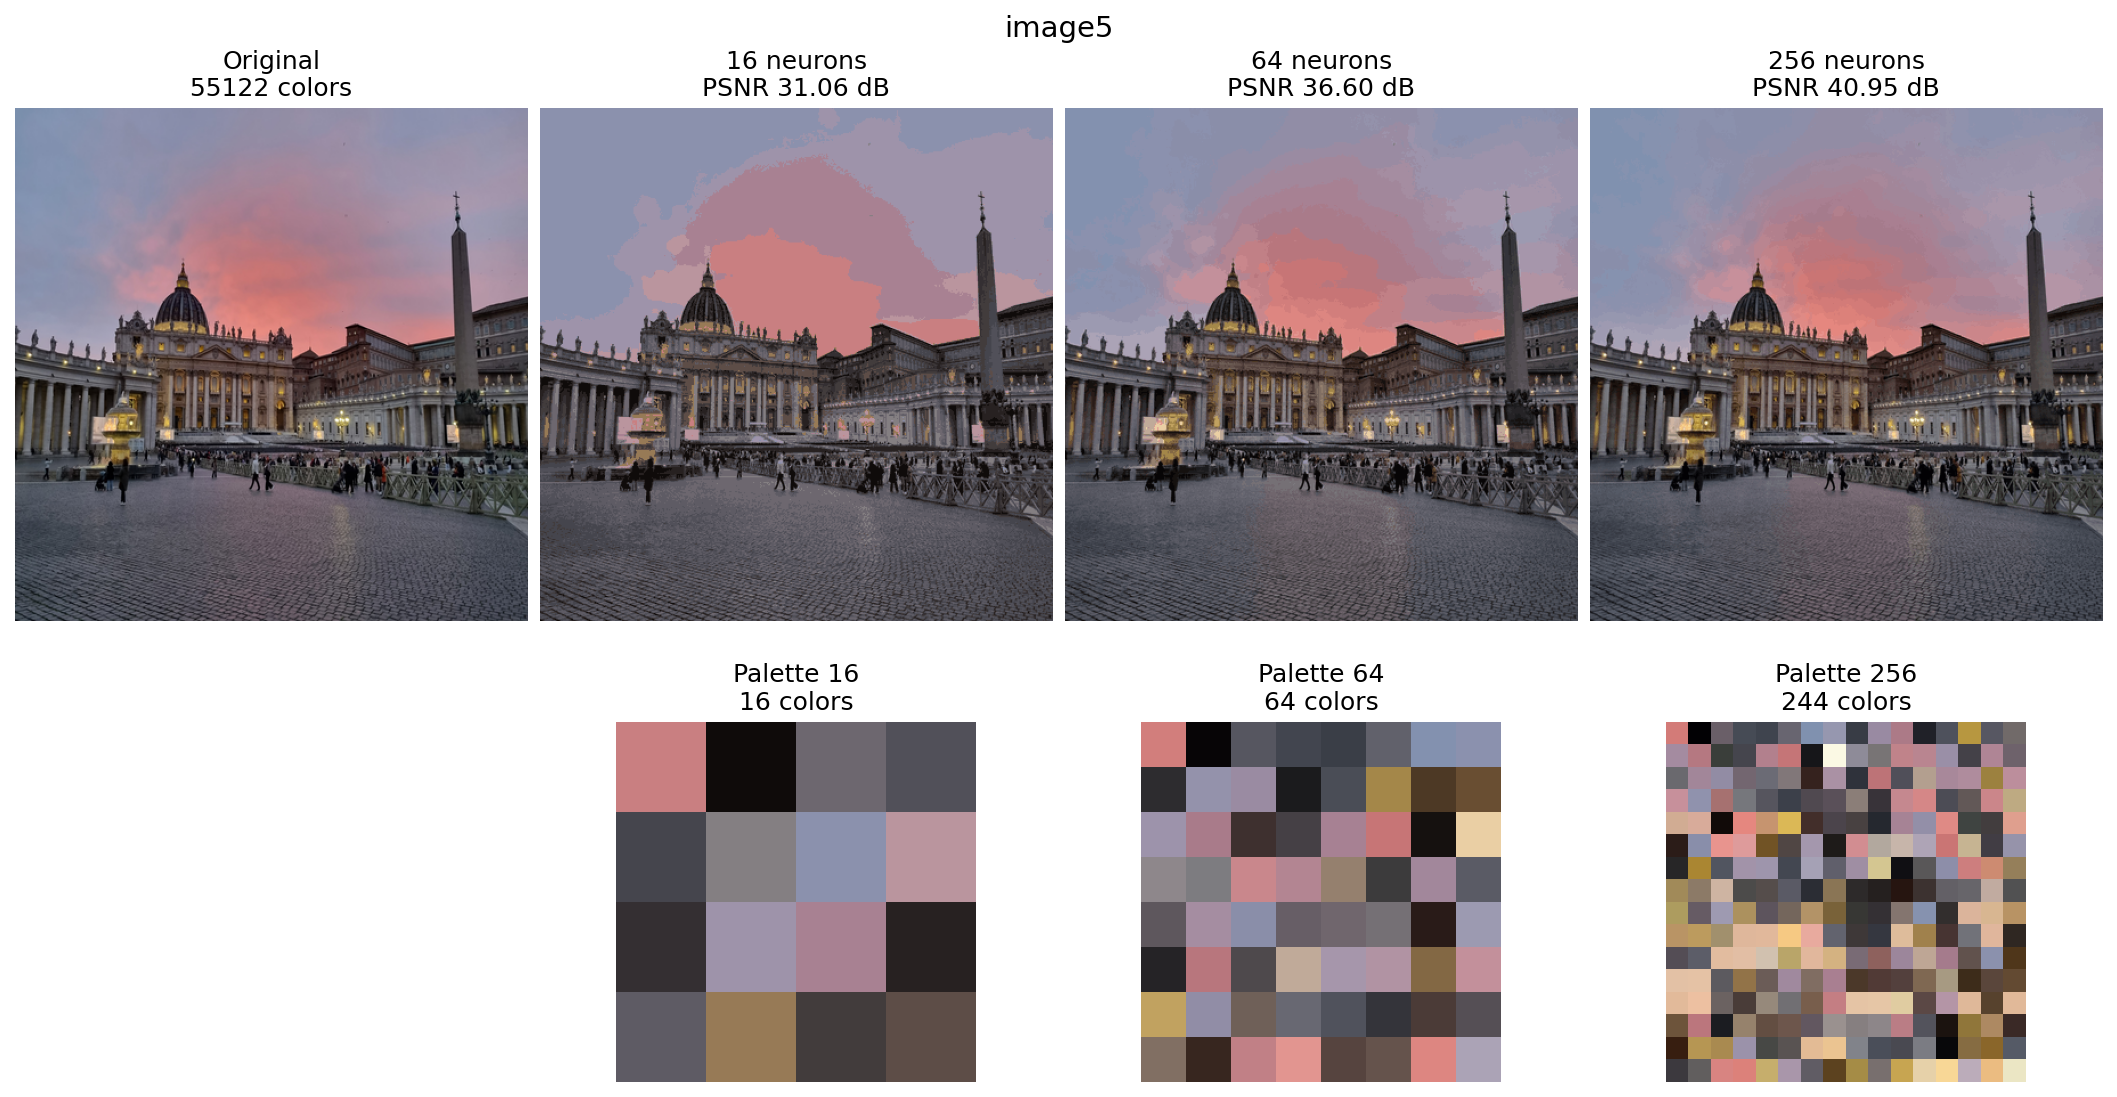
\includegraphics[width=\textwidth]{../gng/results_gng/image5.png}
\caption{Reconstruções via GNG em \texttt{image5}, alcançando o ápice de fidelidade com $41{,}38\,\mathrm{dB}$.}
\label{fig:gng-5}
\end{figure}

\begin{figure}[H]
\centering
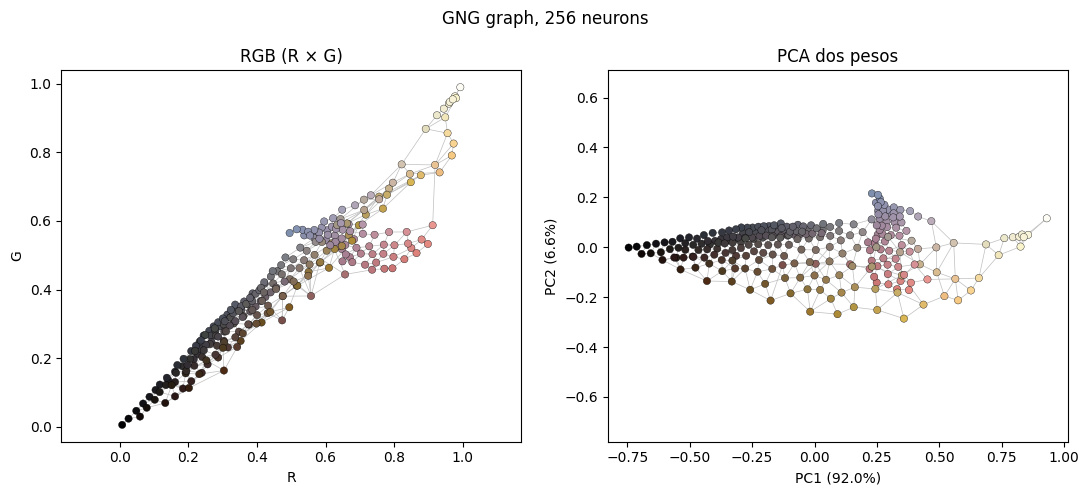
\includegraphics[width=\textwidth]{../gng/results_gng/img5_pca_graph.png}
\caption{Topologia do grafo GNG ($256$ unidades) para \texttt{image5}: à esquerda, projeção $R \times G$; à direita, projeção via PCA, evidenciando o alinhamento da malha ao longo da variedade cromática.}
\label{fig:gng-graph}
\end{figure}

\section{Análise Comparativa}

Ambos os modelos foram submetidos aos mesmos conjuntos de entrada e restritos a tamanhos de codebook idênticos, diferindo fundamentalmente nos princípios de organização topológica. Enquanto a SOM impõe uma geometria rígida prévia sobre a qual projeta os dados, o GNG ajusta localmente a dimensionalidade e conectividade do grafo conforme a distribuição empírica das amostras.

Os resultados compilados na Tabela~\ref{tab:cmp} atestam a superioridade quantitativa consistente do GNG sobre a SOM em todos os $15$ cenários avaliados. A vantagem média em PSNR foi de $+1{,}33\,\mathrm{dB}$ para $16$ cores, $+1{,}58\,\mathrm{dB}$ para $64$ cores e $+1{,}41\,\mathrm{dB}$ para $256$ cores. O ganho mais expressivo ocorreu em \texttt{image5} com $256$ protótipos ($+2{,}26\,\mathrm{dB}$), ao passo que a menor discrepância observou-se em \texttt{image4} para $256$ unidades ($+0{,}83\,\mathrm{dB}$).

\begin{table}[H]
\centering
\caption{Comparação direta de PSNR (dB) entre SOM e GNG em função da capacidade do codebook.}
\label{tab:cmp}
\small
\begin{tabular}{lrrrrrr}
\toprule
 & \multicolumn{2}{c}{$16$ protótipos} & \multicolumn{2}{c}{$64$ protótipos} & \multicolumn{2}{c}{$256$ protótipos} \\
\cmidrule(lr){2-3} \cmidrule(lr){4-5} \cmidrule(lr){6-7}
Imagem & SOM & GNG & SOM & GNG & SOM & GNG \\
\midrule
image1 & 26,10 & 27,16 & 31,63 & 33,14 & 36,59 & 38,16 \\
image2 & 27,54 & 28,85 & 32,96 & 34,70 & 38,34 & 39,68 \\
image3 & 28,18 & 29,17 & 34,24 & 35,19 & 39,26 & 40,29 \\
image4 & 26,88 & 28,72 & 32,58 & 34,13 & 37,90 & 38,73 \\
image5 & 29,72 & 31,16 & 34,53 & 36,68 & 39,12 & 41,38 \\
\midrule
Média  & \textbf{27,68} & \textbf{29,01} & \textbf{33,19} & \textbf{34,77} & \textbf{38,24} & \textbf{39,65} \\
\bottomrule
\end{tabular}
\end{table}

A hierarquia de complexidade das imagens revelou-se congruente entre as duas redes: \texttt{image1} apresentou os maiores índices de erro e menores valores de PSNR em todas as capacidades, reflexo de sua ampla dispersão espectral e transições de iluminação com saturações extremas. Já \texttt{image5} apresentou a melhor convergência para ambos os modelos, favorecida por uma distribuição de cores concentrada ao longo de uma variedade quase unidimensional no espaço RGB. Constatou-se ainda que o efeito da dimensão do codebook supera o do algoritmo adotado: uma SOM com $256$ unidades ($38{,}24\,\mathrm{dB}$) é nitidamente superior a um GNG com $64$ unidades ($34{,}77\,\mathrm{dB}$).

O contraste essencial reside na relação de compromisso (\textit{trade-off}) entre distorção de quantização e interpretabilidade topológica. A restrição rígida da SOM acopla os neurônios de forma a gerar uma ordenação bidimensional intuitiva e contínua do espectro, porém ao custo de limitar a flexibilidade de aproximação e sub-representar populações cromáticas reduzidas (como evidenciado pelo sol de \texttt{image1}, capturado com fidelidade cromática superior pelo GNG com $16$ unidades). Além disso, a atração entre vizinhos na SOM induz redundância em discretizações finitas de $8$ bits, reduzindo a variabilidade efetiva de protótipos.

Em cenários com codebooks densos ($256$ cores), ambas as redes produzem aproximações visuais com alta fidelidade perceptiva, tornando a escolha do algoritmo dependente dos requisitos da aplicação: caso o objetivo primordial seja a minimização estrita da distorção com representação acurada de modas isoladas, o GNG destaca-se como a opção superior; caso a estruturação, indexação espacial ou visualização do espectro cromático seja prioritária, a SOM oferece uma topologia inerentemente organizada.

\end{document}